
\section{Quantitative Results}\label{section:identification}

\subsubsection*{Identification Strategy}

In this section, we estimate the parameters of the model of knowledge diffusion under the optimizing Church's behavior described in Section~\ref{section:theory}, using the data and stylized facts described in Section~\ref{section:data}. We follow a three-step estimation strategy. The first step is to set one parameter following the literature. The second step is to estimate six parameters using a minimum distance estimation procedure, under the assumption that censorship kicks in mid $16^{th}$ century as in the data. The last step is to set one last parameter to match the timing of the introduction of censorship.


\begin{table}[htb]
      \centering % used for centering table
\begin{tabular}{ccccc}
\toprule
$t$         &   years       & rate of censorship $\beta $  & share of censored authors & $\mu_t$ \\
\midrule
1           & 1400-1469     & 0                            & 0                        & 1.000\\
2           & 1470-1539     & 0                            & $m_2\overline{\beta}$    &  0.878\\
3           & 1540-1609     & $\overline{\beta}$           & $m_3\overline{\beta}$    & 0.787\\
4           & 1610-1679     & $\overline{\beta}$           & $m_4\overline{\beta}$    & 0.828\\
5           & 1680-1749     & $\overline{\beta}$           & $m_5\overline{\beta}$    & 0.851\\
\bottomrule
\end{tabular}
\caption{Model Periods}\label{tab:periods}
\end{table}

Before going into the estimation details, we specify the relationship between model periods and their empirical counterpart, see Table~\ref{tab:periods}.
We consider five model periods that correspond to 1400-1469, 1470-1539, 1540-1609, 1610-1679, and 1680-1749. We made this choice following four criteria. First, we want each period to correspond to an equal number of years. Second, we want to stop in 1750 as the Church might have lost the capacity to censor after this date.\footnote{\citeN{putnam1906} claims that censorship exerted the largest influence between 1550 to 1750.} Third, we want a year close to 1544 (first edition of the Index) to be the threshold between two consecutive model periods. In this way, we can claim that censorship started in the second of these two periods. Finally, we don't want each period to be too short because the number of authors per period would be small, causing the moments' standard errors to be large. A robustness analysis with ten periods instead of five is proposed in Appendix~\ref{O-app:robust}.




Table~\ref{tab:periods} shows in parallel the censorship rate and the share of censored authors, to stress that censorship in period 3 affects books written in period 2.
The process for $\mu$ is taken from the annual GDP per capita series offered by \citeN{malanima2011long} and \citeN{bolt2020maddison}. $\mu_t$ is obtained by averaging GDP per capita over the 70 calendar years corresponding to each model period $t$. Values are normalized to have $\mu_1=1$.

\textbf{Preset Parameter.} We set the discount factor $\delta$ to 0.06, which corresponds to a quarterly discount factor of $0.99$: $0.06\approx0.99^{280}$. This parameter's role is minimal: conditionally on censorship starting on $t=3$, it does not affect dynamics.

\textbf{Minimum Distance Estimation.} We estimate the vector of six parameters
$$\vartheta=[k^C_1,k^R_1,\theta,\overline{\beta},\nu,p]$$
 using a minimum distance estimation procedure. The parameters are identified by minimizing the distance between 14 empirical and theoretical moments, implying thus 8 (=14-6) over\-identifying restrictions.  The first  moments are based on the distribution of the quality of all authors, $q_{it}$, obtained by drawing with probability $m_t$ from the distribution of $q^R_t$ (i.e. a Fréchet($(k_t^R)^\theta,1/\theta$)) and with probability $(1-m_t)$  from the distribution of $q^C_t$.  Five moments are the median\footnote{We target the median instead of the mean because it is less sensitive to outliers.} of the quality of all authors $Q_2(q_t)$, and five other moments are their  $75^{th}$ percentile $Q_3(q_t)$. The last four moments are the share of censored authors $m_t \overline{\beta}$ for $t=2,3,4,5$.

The above estimation problem belongs to the family of the Simulated Method of Moments \cite{mcfadden1989method}, a structural estimation technique to be applied when the theoretical moments obtain from simulating the model. Remark that we refrain from targeting separately moments based on censored vs. non-censored authors. These moments will rather be used to evaluate the quality of our estimation.

Our six parameters are expected to influence all moments (except $\nu$ which does not affect $m_t\overline{\beta}$). But we can still think that some moments are more important than others for identifying specific parameters. Parameters $k^C_1,k^R_1$ are  identified by moment $m_2 \overline{\beta}$ (which depends on $m_1 \overline{\beta}$ through Equation~(\ref{eq:lawm}))  and by the median of the distribution of $q_{i1}$. Parameter $\nu$ is identified by the growth rate of overall quality. Parameter $p$ is  identified by the average share of censored authors $m_t \overline{\beta}$ over time (see Equation~(\ref{eq:sharer2})).  Parameter $\overline{\beta}$ influences the speed at which $m_t$ converges (Equation~(\ref{eq:lawm})), and is thus identified by the dynamics of the share of censored authors. Parameter $\theta$ governs the shape of the Fr\'echet distribution of knowledge quality and is identified by the $75^{th}$ percentile of the quality distribution.




\textbf{Parameter set a posteriori.}  We set parameter $\psi$ such that censorship starts in $t=3$ as in the data. Parameter $\psi$ has no impact on knowledge dynamics conditional on censorship starting in a defined year. See Appendix~\ref{O-app:dpsi} for more details on the calibration of $\psi$.





\subsubsection*{Estimation Results}

We list the identified parameters and their standard errors in Table~\ref{table:param}. The estimation delivers $k^R_1>k^C_1$: this implies that the quality of censored authors is higher than non-censored authors, which is consistent with data even if the relative quality by sector is not among the targeted moments. The productivity of books $\theta$ equals 0.34: this is slightly lower than the value (0.5) used by \citeN{lucas2009}. Our estimate is lower because the dispersion in log publications is lower than the one in earnings observed in modern U.S. data, which is the target of \citeN{lucas2009}.
 The relative price of revolutionary books $p$ equals $0.51$. This insures that the initial share of revolutionary authors is not too large, even if they have a much higher quality than compliant scholars.\footnote{For example, if $p$ was equal to 1, the share of revolutionary authors would converge to 1 very fast: as a result, the share of censored authors would converge to $\overline{\beta}$ and stay constant, unlike in the data.} Parameter $\nu$ insures that knowledge quality would have kept growing if censorship was never introduced. The rate of censorship $\overline{\beta}$ that the Church imposes equals 19\%.

%%%%TABLE PARAMETERS%%%%%
%UPDATED 29 AUG 2022=========================================================================================================================
\begin{table}[htpb]
      \centering % used for centering table
      \begin{tabular}{@{\extracolsep{5pt}}l c c c c} 
      \toprule%inserts double horizontal lines
      \rule{-4pt}{2.5ex}
       Estimated Parameters &  & Value & Standard Errors & Target  \\ [0.05ex] % inserts table
        %heading
      \midrule % inserts single horizontal line
      \rule{-4pt}{2.5ex}
      Compliant knowledge in 1  & $k^C_1$   & 16.5 & 1.2  &  $\Omega(\vartheta)$  \\[0.15ex]
      Rev. knowledge in 1  & $k^R_1$   & 125.1 & 10.73  & $\Omega(\vartheta)$ \\[0.15ex]
      Productivity of books  & $\theta$   & 0.34 &  0.017  & $\Omega(\vartheta)$\\[0.15ex]
      Max Censorship  & $\overline{\beta}$   & 0.19 &  0.015 & $\Omega(\vartheta)$\\[0.15ex]
      Knowledge Growth   & $\nu$   & 1.4 &  0.071  & $\Omega(\vartheta)$\\[0.15ex]
      Price of rev. books   & $p$   & 0.51 &  0.019  & $\Omega(\vartheta)$\\[0.15ex]
      \bottomrule
      	\multicolumn{5}{l}{\footnotesize Note: for more detail on the computation of standard errors see Appendix~\ref{O-app:dest}}
      \end{tabular}
       \caption{Identification of Parameters}
      \label{table:param}
      \end{table}




%UPDATED 29 AUG 2022=========================================================================================================================
\begin{figure}[p]	
\hspace{0mm}
\parbox{.49\textwidth}{
		\centering
		{Overall scholars quality:\\ \textcolor{red}{median $Q_2(q_t)$}, \textcolor{blue}{$75^{th}$ percentile $Q_3(q_t)$}}

\scalebox{0.55}{% Created by tikzDevice version 0.12.3.1 on 2022-09-19 21:45:14
% !TEX encoding = UTF-8 Unicode
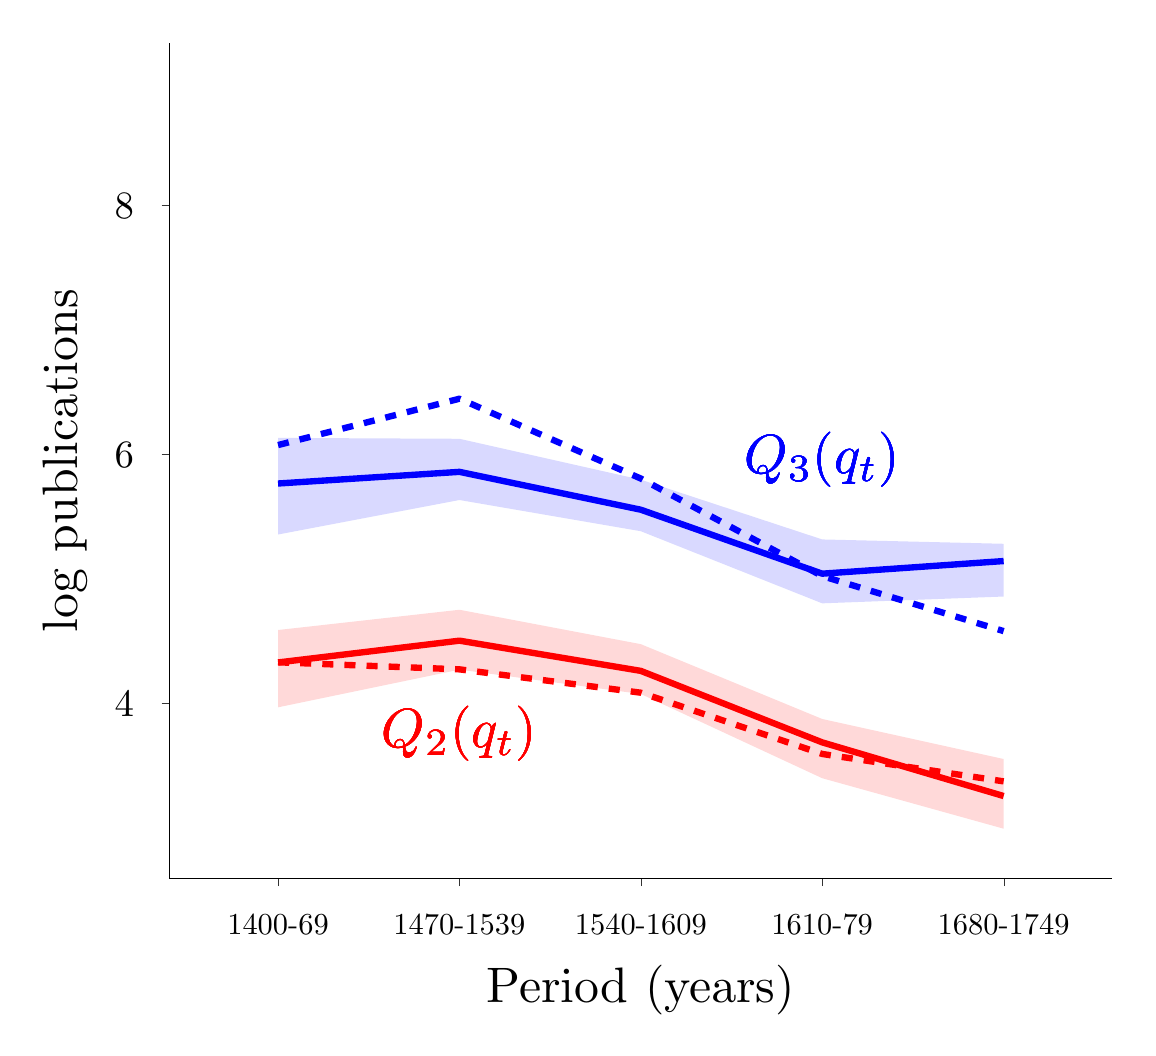
\begin{tikzpicture}[x=1pt,y=1pt]
\definecolor{fillColor}{RGB}{255,255,255}
\path[use as bounding box,fill=fillColor,fill opacity=0.00] (0,0) rectangle (397.48,361.35);
\begin{scope}
\path[clip] (  0.00,  0.00) rectangle (397.48,361.35);
\definecolor{drawColor}{RGB}{255,255,255}
\definecolor{fillColor}{RGB}{255,255,255}

\path[draw=drawColor,line width= 0.1pt,line join=round,line cap=round,fill=fillColor] (  0.00,  0.00) rectangle (397.48,361.35);
\end{scope}
\begin{scope}
\path[clip] ( 51.14, 53.86) rectangle (391.98,355.85);
\definecolor{fillColor}{RGB}{255,255,255}

\path[fill=fillColor] ( 51.14, 53.86) rectangle (391.98,355.85);
\definecolor{fillColor}{RGB}{255,0,0}

\path[fill=fillColor,fill opacity=0.15] ( 90.47,143.69) --
	(156.02,151.01) --
	(221.56,138.58) --
	(287.11,111.54) --
	(352.66, 97.08) --
	(352.66, 71.90) --
	(287.11, 90.14) --
	(221.56,120.58) --
	(156.02,129.37) --
	( 90.47,115.76) --
	cycle;

\path[] ( 90.47,143.69) --
	(156.02,151.01) --
	(221.56,138.58) --
	(287.11,111.54) --
	(352.66, 97.08);

\path[] (352.66, 71.90) --
	(287.11, 90.14) --
	(221.56,120.58) --
	(156.02,129.37) --
	( 90.47,115.76);
\definecolor{drawColor}{RGB}{255,0,0}

\path[draw=drawColor,line width= 2.3pt,line join=round] ( 90.47,131.97) --
	(156.02,139.84) --
	(221.56,128.92) --
	(287.11,103.09) --
	(352.66, 83.70);

\path[draw=drawColor,line width= 2.3pt,dash pattern=on 4pt off 4pt ,line join=round] ( 90.47,132.03) --
	(156.02,129.48) --
	(221.56,121.04) --
	(287.11, 98.90) --
	(352.66, 89.00);
\definecolor{fillColor}{RGB}{0,0,255}

\path[fill=fillColor,fill opacity=0.15] ( 90.47,213.11) --
	(156.02,212.79) --
	(221.56,198.01) --
	(287.11,176.42) --
	(352.66,174.85) --
	(352.66,155.79) --
	(287.11,153.33) --
	(221.56,179.39) --
	(156.02,190.67) --
	( 90.47,178.20) --
	cycle;

\path[] ( 90.47,213.11) --
	(156.02,212.79) --
	(221.56,198.01) --
	(287.11,176.42) --
	(352.66,174.85);

\path[] (352.66,155.79) --
	(287.11,153.33) --
	(221.56,179.39) --
	(156.02,190.67) --
	( 90.47,178.20);
\definecolor{drawColor}{RGB}{0,0,255}

\path[draw=drawColor,line width= 2.3pt,line join=round] ( 90.47,196.63) --
	(156.02,200.84) --
	(221.56,187.16) --
	(287.11,164.05) --
	(352.66,168.61);

\path[draw=drawColor,line width= 2.3pt,dash pattern=on 4pt off 4pt ,line join=round] ( 90.47,210.52) --
	(156.02,227.27) --
	(221.56,198.42) --
	(287.11,163.18) --
	(352.66,143.30);

\node[text=drawColor,anchor=base,inner sep=0pt, outer sep=0pt, scale=  1.99] at (287.11,200.25) {$Q_3(q_t)$};

\node[text=drawColor,anchor=base,inner sep=0pt, outer sep=0pt, scale=  1.99] at (287.11,200.25) {$Q_3(q_t)$};

\node[text=drawColor,anchor=base,inner sep=0pt, outer sep=0pt, scale=  1.99] at (287.11,200.25) {$Q_3(q_t)$};

\node[text=drawColor,anchor=base,inner sep=0pt, outer sep=0pt, scale=  1.99] at (287.11,200.25) {$Q_3(q_t)$};

\node[text=drawColor,anchor=base,inner sep=0pt, outer sep=0pt, scale=  1.99] at (287.11,200.25) {$Q_3(q_t)$};
\definecolor{drawColor}{RGB}{255,0,0}

\node[text=drawColor,anchor=base,inner sep=0pt, outer sep=0pt, scale=  1.99] at (156.02,101.23) {$Q_2(q_t)$};

\node[text=drawColor,anchor=base,inner sep=0pt, outer sep=0pt, scale=  1.99] at (156.02,101.23) {$Q_2(q_t)$};

\node[text=drawColor,anchor=base,inner sep=0pt, outer sep=0pt, scale=  1.99] at (156.02,101.23) {$Q_2(q_t)$};

\node[text=drawColor,anchor=base,inner sep=0pt, outer sep=0pt, scale=  1.99] at (156.02,101.23) {$Q_2(q_t)$};

\node[text=drawColor,anchor=base,inner sep=0pt, outer sep=0pt, scale=  1.99] at (156.02,101.23) {$Q_2(q_t)$};
\end{scope}
\begin{scope}
\path[clip] (  0.00,  0.00) rectangle (397.48,361.35);
\definecolor{drawColor}{RGB}{0,0,0}

\path[draw=drawColor,line width= 0.1pt,line join=round] ( 51.14, 53.86) --
	( 51.14,355.85);
\end{scope}
\begin{scope}
\path[clip] (  0.00,  0.00) rectangle (397.48,361.35);
\definecolor{drawColor}{RGB}{0,0,0}

\node[text=drawColor,anchor=base east,inner sep=0pt, outer sep=0pt, scale=  1.40] at ( 38.39,112.27) {4};

\node[text=drawColor,anchor=base east,inner sep=0pt, outer sep=0pt, scale=  1.40] at ( 38.39,202.28) {6};

\node[text=drawColor,anchor=base east,inner sep=0pt, outer sep=0pt, scale=  1.40] at ( 38.39,292.30) {8};
\end{scope}
\begin{scope}
\path[clip] (  0.00,  0.00) rectangle (397.48,361.35);
\definecolor{drawColor}{gray}{0.20}

\path[draw=drawColor,line width= 0.1pt,line join=round] ( 48.39,117.09) --
	( 51.14,117.09);

\path[draw=drawColor,line width= 0.1pt,line join=round] ( 48.39,207.11) --
	( 51.14,207.11);

\path[draw=drawColor,line width= 0.1pt,line join=round] ( 48.39,297.12) --
	( 51.14,297.12);
\end{scope}
\begin{scope}
\path[clip] (  0.00,  0.00) rectangle (397.48,361.35);
\definecolor{drawColor}{RGB}{0,0,0}

\path[draw=drawColor,line width= 0.1pt,line join=round] ( 51.14, 53.86) --
	(391.98, 53.86);
\end{scope}
\begin{scope}
\path[clip] (  0.00,  0.00) rectangle (397.48,361.35);
\definecolor{drawColor}{gray}{0.20}

\path[draw=drawColor,line width= 0.1pt,line join=round] ( 90.47, 51.11) --
	( 90.47, 53.86);

\path[draw=drawColor,line width= 0.1pt,line join=round] (156.02, 51.11) --
	(156.02, 53.86);

\path[draw=drawColor,line width= 0.1pt,line join=round] (221.56, 51.11) --
	(221.56, 53.86);

\path[draw=drawColor,line width= 0.1pt,line join=round] (287.11, 51.11) --
	(287.11, 53.86);

\path[draw=drawColor,line width= 0.1pt,line join=round] (352.66, 51.11) --
	(352.66, 53.86);
\end{scope}
\begin{scope}
\path[clip] (  0.00,  0.00) rectangle (397.48,361.35);
\definecolor{drawColor}{RGB}{0,0,0}

\node[text=drawColor,anchor=base,inner sep=0pt, outer sep=0pt, scale=  1.10] at ( 90.47, 33.53) {1400-69};

\node[text=drawColor,anchor=base,inner sep=0pt, outer sep=0pt, scale=  1.10] at (156.02, 33.53) {1470-1539};

\node[text=drawColor,anchor=base,inner sep=0pt, outer sep=0pt, scale=  1.10] at (221.56, 33.53) {1540-1609};

\node[text=drawColor,anchor=base,inner sep=0pt, outer sep=0pt, scale=  1.10] at (287.11, 33.53) {1610-79};

\node[text=drawColor,anchor=base,inner sep=0pt, outer sep=0pt, scale=  1.10] at (352.66, 33.53) {1680-1749};
\end{scope}
\begin{scope}
\path[clip] (  0.00,  0.00) rectangle (397.48,361.35);
\definecolor{drawColor}{RGB}{0,0,0}

\node[text=drawColor,anchor=base,inner sep=0pt, outer sep=0pt, scale=  1.80] at (221.56,  9.00) {Period (years)};
\end{scope}
\begin{scope}
\path[clip] (  0.00,  0.00) rectangle (397.48,361.35);
\definecolor{drawColor}{RGB}{0,0,0}

\node[text=drawColor,rotate= 90.00,anchor=base,inner sep=0pt, outer sep=0pt, scale=  1.80] at ( 17.90,204.86) {log publications};
\end{scope}
\end{tikzpicture}
}
}\hspace{-6mm}
\parbox{.49\textwidth}{
		\centering
{Share of censored scholars $\overline{\beta}m_t$\\
\textcolor{white}{a}}

\scalebox{0.55}{% Created by tikzDevice version 0.12.3.1 on 2022-09-19 22:27:54
% !TEX encoding = UTF-8 Unicode
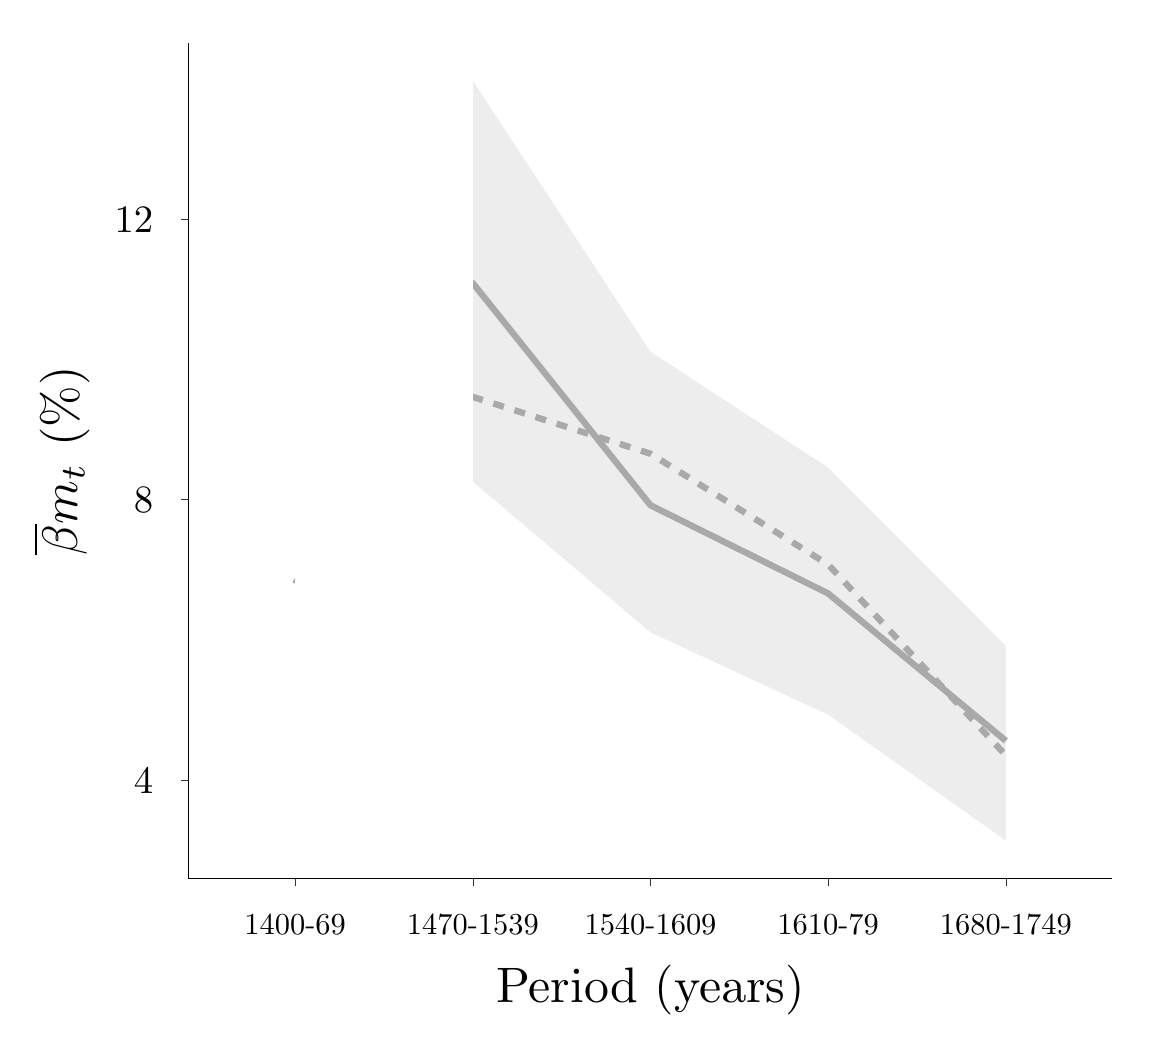
\begin{tikzpicture}[x=1pt,y=1pt]
\definecolor{fillColor}{RGB}{255,255,255}
\path[use as bounding box,fill=fillColor,fill opacity=0.00] (0,0) rectangle (397.48,361.35);
\begin{scope}
\path[clip] (  0.00,  0.00) rectangle (397.48,361.35);
\definecolor{drawColor}{RGB}{255,255,255}
\definecolor{fillColor}{RGB}{255,255,255}

\path[draw=drawColor,line width= 0.1pt,line join=round,line cap=round,fill=fillColor] (  0.00,  0.00) rectangle (397.48,361.35);
\end{scope}
\begin{scope}
\path[clip] ( 58.14, 53.86) rectangle (391.98,355.85);
\definecolor{fillColor}{RGB}{255,255,255}

\path[fill=fillColor] ( 58.14, 53.86) rectangle (391.98,355.85);
\definecolor{fillColor}{RGB}{169,169,169}

\path[fill=fillColor,fill opacity=0.20] ( 96.66,263.42) --
	(160.86,342.12) --
	(225.06,244.23) --
	(289.26,202.36) --
	(353.46,137.94) --
	(353.46, 67.59) --
	(289.26,113.10) --
	(225.06,142.83) --
	(160.86,197.32) --
	( 96.66, 75.91) --
	cycle;

\path[] ( 96.66,263.42) --
	(160.86,342.12) --
	(225.06,244.23) --
	(289.26,202.36) --
	(353.46,137.94);

\path[] (353.46, 67.59) --
	(289.26,113.10) --
	(225.06,142.83) --
	(160.86,197.32) --
	( 96.66, 75.91);
\definecolor{drawColor}{RGB}{169,169,169}

\path[draw=drawColor,line width= 2.3pt,line join=round] ( 96.66,160.39) --
	(160.86,269.05) --
	(225.06,188.77) --
	(289.26,156.89) --
	(353.46,103.64);

\path[draw=drawColor,line width= 2.3pt,dash pattern=on 4pt off 4pt ,line join=round] ( 96.66,226.06) --
	(160.86,227.93) --
	(225.06,207.39) --
	(289.26,167.35) --
	(353.46, 98.39);
\definecolor{fillColor}{RGB}{255,255,255}

\path[fill=fillColor] ( 96.66, 53.86) rectangle (160.86,355.85);

\path[fill=fillColor] ( 96.66, 53.86) rectangle (160.86,355.85);

\path[fill=fillColor] ( 96.66, 53.86) rectangle (160.86,355.85);

\path[fill=fillColor] ( 96.66, 53.86) rectangle (160.86,355.85);

\path[fill=fillColor] ( 96.66, 53.86) rectangle (160.86,355.85);
\end{scope}
\begin{scope}
\path[clip] (  0.00,  0.00) rectangle (397.48,361.35);
\definecolor{drawColor}{RGB}{0,0,0}

\path[draw=drawColor,line width= 0.1pt,line join=round] ( 58.14, 53.86) --
	( 58.14,355.85);
\end{scope}
\begin{scope}
\path[clip] (  0.00,  0.00) rectangle (397.48,361.35);
\definecolor{drawColor}{RGB}{0,0,0}

\node[text=drawColor,anchor=base east,inner sep=0pt, outer sep=0pt, scale=  1.40] at ( 45.39, 84.70) {4};

\node[text=drawColor,anchor=base east,inner sep=0pt, outer sep=0pt, scale=  1.40] at ( 45.39,186.09) {8};

\node[text=drawColor,anchor=base east,inner sep=0pt, outer sep=0pt, scale=  1.40] at ( 45.39,287.49) {12};
\end{scope}
\begin{scope}
\path[clip] (  0.00,  0.00) rectangle (397.48,361.35);
\definecolor{drawColor}{gray}{0.20}

\path[draw=drawColor,line width= 0.1pt,line join=round] ( 55.39, 89.52) --
	( 58.14, 89.52);

\path[draw=drawColor,line width= 0.1pt,line join=round] ( 55.39,190.91) --
	( 58.14,190.91);

\path[draw=drawColor,line width= 0.1pt,line join=round] ( 55.39,292.31) --
	( 58.14,292.31);
\end{scope}
\begin{scope}
\path[clip] (  0.00,  0.00) rectangle (397.48,361.35);
\definecolor{drawColor}{RGB}{0,0,0}

\path[draw=drawColor,line width= 0.1pt,line join=round] ( 58.14, 53.86) --
	(391.98, 53.86);
\end{scope}
\begin{scope}
\path[clip] (  0.00,  0.00) rectangle (397.48,361.35);
\definecolor{drawColor}{gray}{0.20}

\path[draw=drawColor,line width= 0.1pt,line join=round] ( 96.66, 51.11) --
	( 96.66, 53.86);

\path[draw=drawColor,line width= 0.1pt,line join=round] (160.86, 51.11) --
	(160.86, 53.86);

\path[draw=drawColor,line width= 0.1pt,line join=round] (225.06, 51.11) --
	(225.06, 53.86);

\path[draw=drawColor,line width= 0.1pt,line join=round] (289.26, 51.11) --
	(289.26, 53.86);

\path[draw=drawColor,line width= 0.1pt,line join=round] (353.46, 51.11) --
	(353.46, 53.86);
\end{scope}
\begin{scope}
\path[clip] (  0.00,  0.00) rectangle (397.48,361.35);
\definecolor{drawColor}{RGB}{0,0,0}

\node[text=drawColor,anchor=base,inner sep=0pt, outer sep=0pt, scale=  1.10] at ( 96.66, 33.53) {1400-69};

\node[text=drawColor,anchor=base,inner sep=0pt, outer sep=0pt, scale=  1.10] at (160.86, 33.53) {1470-1539};

\node[text=drawColor,anchor=base,inner sep=0pt, outer sep=0pt, scale=  1.10] at (225.06, 33.53) {1540-1609};

\node[text=drawColor,anchor=base,inner sep=0pt, outer sep=0pt, scale=  1.10] at (289.26, 33.53) {1610-79};

\node[text=drawColor,anchor=base,inner sep=0pt, outer sep=0pt, scale=  1.10] at (353.46, 33.53) {1680-1749};
\end{scope}
\begin{scope}
\path[clip] (  0.00,  0.00) rectangle (397.48,361.35);
\definecolor{drawColor}{RGB}{0,0,0}

\node[text=drawColor,anchor=base,inner sep=0pt, outer sep=0pt, scale=  1.80] at (225.06,  9.00) {Period (years)};
\end{scope}
\begin{scope}
\path[clip] (  0.00,  0.00) rectangle (397.48,361.35);
\definecolor{drawColor}{RGB}{0,0,0}

\node[text=drawColor,rotate= 90.00,anchor=base,inner sep=0pt, outer sep=0pt, scale=  1.80] at ( 17.90,204.86) {$\overline{\beta}m_t$ (\%)};
\end{scope}
\end{tikzpicture}
}
}

\vspace{10mm}
\hspace{0mm}
\parbox{.49\textwidth}{
		\centering
{Censored scholars quality:\\ \textcolor{red}{median $Q_2(q_t^R)$}, \textcolor{blue}{$75^{th}$ percentile $Q_3(q_t^R)$}}

\scalebox{0.55}{% Created by tikzDevice version 0.12.3.1 on 2022-09-19 22:27:53
% !TEX encoding = UTF-8 Unicode
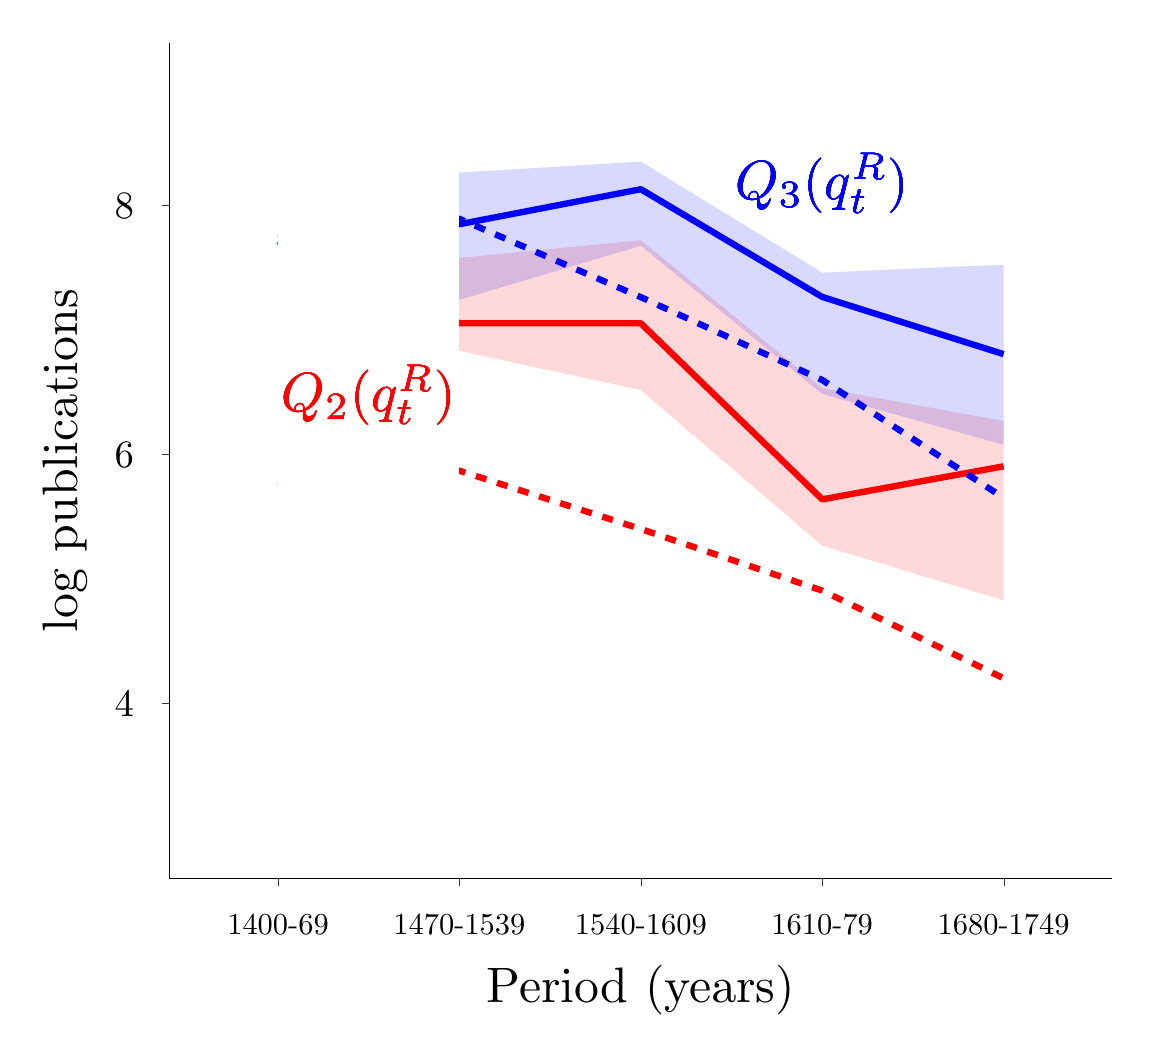
\begin{tikzpicture}[x=1pt,y=1pt]
\definecolor{fillColor}{RGB}{255,255,255}
\path[use as bounding box,fill=fillColor,fill opacity=0.00] (0,0) rectangle (397.48,361.35);
\begin{scope}
\path[clip] (  0.00,  0.00) rectangle (397.48,361.35);
\definecolor{drawColor}{RGB}{255,255,255}
\definecolor{fillColor}{RGB}{255,255,255}

\path[draw=drawColor,line width= 0.1pt,line join=round,line cap=round,fill=fillColor] (  0.00,  0.00) rectangle (397.48,361.35);
\end{scope}
\begin{scope}
\path[clip] ( 51.14, 53.86) rectangle (391.98,355.85);
\definecolor{fillColor}{RGB}{255,255,255}

\path[fill=fillColor] ( 51.14, 53.86) rectangle (391.98,355.85);
\definecolor{fillColor}{RGB}{255,0,0}

\path[fill=fillColor,fill opacity=0.15] ( 90.47,292.14) --
	(156.02,278.15) --
	(221.56,284.53) --
	(287.11,231.13) --
	(352.66,219.22) --
	(352.66,154.37) --
	(287.11,174.15) --
	(221.56,230.40) --
	(156.02,244.55) --
	( 90.47,254.76) --
	cycle;

\path[] ( 90.47,292.14) --
	(156.02,278.15) --
	(221.56,284.53) --
	(287.11,231.13) --
	(352.66,219.22);

\path[] (352.66,154.37) --
	(287.11,174.15) --
	(221.56,230.40) --
	(156.02,244.55) --
	( 90.47,254.76);
\definecolor{drawColor}{RGB}{255,0,0}

\path[draw=drawColor,line width= 2.3pt,line join=round] ( 90.47,284.23) --
	(156.02,254.56) --
	(221.56,254.52) --
	(287.11,190.91) --
	(352.66,202.85);

\path[draw=drawColor,line width= 2.3pt,dash pattern=on 4pt off 4pt ,line join=round] ( 90.47,195.87) --
	(156.02,201.25) --
	(221.56,180.20) --
	(287.11,157.93) --
	(352.66,126.27);
\definecolor{fillColor}{RGB}{0,0,255}

\path[fill=fillColor,fill opacity=0.15] ( 90.47,325.49) --
	(156.02,308.99) --
	(221.56,312.95) --
	(287.11,272.84) --
	(352.66,275.70) --
	(352.66,210.60) --
	(287.11,228.99) --
	(221.56,282.55) --
	(156.02,262.97) --
	( 90.47,278.47) --
	cycle;

\path[] ( 90.47,325.49) --
	(156.02,308.99) --
	(221.56,312.95) --
	(287.11,272.84) --
	(352.66,275.70);

\path[] (352.66,210.60) --
	(287.11,228.99) --
	(221.56,282.55) --
	(156.02,262.97) --
	( 90.47,278.47);
\definecolor{drawColor}{RGB}{0,0,255}

\path[draw=drawColor,line width= 2.3pt,line join=round] ( 90.47,291.49) --
	(156.02,290.33) --
	(221.56,302.97) --
	(287.11,264.05) --
	(352.66,243.37);

\path[draw=drawColor,line width= 2.3pt,dash pattern=on 4pt off 4pt ,line join=round] ( 90.47,285.04) --
	(156.02,292.27) --
	(221.56,263.97) --
	(287.11,234.03) --
	(352.66,191.46);
\definecolor{fillColor}{RGB}{255,255,255}

\path[fill=fillColor] ( 90.47, 53.86) rectangle (156.02,355.85);

\path[fill=fillColor] ( 90.47, 53.86) rectangle (156.02,355.85);

\path[fill=fillColor] ( 90.47, 53.86) rectangle (156.02,355.85);

\path[fill=fillColor] ( 90.47, 53.86) rectangle (156.02,355.85);

\path[fill=fillColor] ( 90.47, 53.86) rectangle (156.02,355.85);

\node[text=drawColor,anchor=base,inner sep=0pt, outer sep=0pt, scale=  1.99] at (287.11,299.26) {$Q_3(q_t^R)$};

\node[text=drawColor,anchor=base,inner sep=0pt, outer sep=0pt, scale=  1.99] at (287.11,299.26) {$Q_3(q_t^R)$};

\node[text=drawColor,anchor=base,inner sep=0pt, outer sep=0pt, scale=  1.99] at (287.11,299.26) {$Q_3(q_t^R)$};

\node[text=drawColor,anchor=base,inner sep=0pt, outer sep=0pt, scale=  1.99] at (287.11,299.26) {$Q_3(q_t^R)$};

\node[text=drawColor,anchor=base,inner sep=0pt, outer sep=0pt, scale=  1.99] at (287.11,299.26) {$Q_3(q_t^R)$};
\definecolor{drawColor}{RGB}{255,0,0}

\node[text=drawColor,anchor=base,inner sep=0pt, outer sep=0pt, scale=  1.99] at (123.25,222.75) {$Q_2(q_t^R)$};

\node[text=drawColor,anchor=base,inner sep=0pt, outer sep=0pt, scale=  1.99] at (123.25,222.75) {$Q_2(q_t^R)$};

\node[text=drawColor,anchor=base,inner sep=0pt, outer sep=0pt, scale=  1.99] at (123.25,222.75) {$Q_2(q_t^R)$};

\node[text=drawColor,anchor=base,inner sep=0pt, outer sep=0pt, scale=  1.99] at (123.25,222.75) {$Q_2(q_t^R)$};

\node[text=drawColor,anchor=base,inner sep=0pt, outer sep=0pt, scale=  1.99] at (123.25,222.75) {$Q_2(q_t^R)$};
\end{scope}
\begin{scope}
\path[clip] (  0.00,  0.00) rectangle (397.48,361.35);
\definecolor{drawColor}{RGB}{0,0,0}

\path[draw=drawColor,line width= 0.1pt,line join=round] ( 51.14, 53.86) --
	( 51.14,355.85);
\end{scope}
\begin{scope}
\path[clip] (  0.00,  0.00) rectangle (397.48,361.35);
\definecolor{drawColor}{RGB}{0,0,0}

\node[text=drawColor,anchor=base east,inner sep=0pt, outer sep=0pt, scale=  1.40] at ( 38.39,112.27) {4};

\node[text=drawColor,anchor=base east,inner sep=0pt, outer sep=0pt, scale=  1.40] at ( 38.39,202.28) {6};

\node[text=drawColor,anchor=base east,inner sep=0pt, outer sep=0pt, scale=  1.40] at ( 38.39,292.30) {8};
\end{scope}
\begin{scope}
\path[clip] (  0.00,  0.00) rectangle (397.48,361.35);
\definecolor{drawColor}{gray}{0.20}

\path[draw=drawColor,line width= 0.1pt,line join=round] ( 48.39,117.09) --
	( 51.14,117.09);

\path[draw=drawColor,line width= 0.1pt,line join=round] ( 48.39,207.11) --
	( 51.14,207.11);

\path[draw=drawColor,line width= 0.1pt,line join=round] ( 48.39,297.12) --
	( 51.14,297.12);
\end{scope}
\begin{scope}
\path[clip] (  0.00,  0.00) rectangle (397.48,361.35);
\definecolor{drawColor}{RGB}{0,0,0}

\path[draw=drawColor,line width= 0.1pt,line join=round] ( 51.14, 53.86) --
	(391.98, 53.86);
\end{scope}
\begin{scope}
\path[clip] (  0.00,  0.00) rectangle (397.48,361.35);
\definecolor{drawColor}{gray}{0.20}

\path[draw=drawColor,line width= 0.1pt,line join=round] ( 90.47, 51.11) --
	( 90.47, 53.86);

\path[draw=drawColor,line width= 0.1pt,line join=round] (156.02, 51.11) --
	(156.02, 53.86);

\path[draw=drawColor,line width= 0.1pt,line join=round] (221.56, 51.11) --
	(221.56, 53.86);

\path[draw=drawColor,line width= 0.1pt,line join=round] (287.11, 51.11) --
	(287.11, 53.86);

\path[draw=drawColor,line width= 0.1pt,line join=round] (352.66, 51.11) --
	(352.66, 53.86);
\end{scope}
\begin{scope}
\path[clip] (  0.00,  0.00) rectangle (397.48,361.35);
\definecolor{drawColor}{RGB}{0,0,0}

\node[text=drawColor,anchor=base,inner sep=0pt, outer sep=0pt, scale=  1.10] at ( 90.47, 33.53) {1400-69};

\node[text=drawColor,anchor=base,inner sep=0pt, outer sep=0pt, scale=  1.10] at (156.02, 33.53) {1470-1539};

\node[text=drawColor,anchor=base,inner sep=0pt, outer sep=0pt, scale=  1.10] at (221.56, 33.53) {1540-1609};

\node[text=drawColor,anchor=base,inner sep=0pt, outer sep=0pt, scale=  1.10] at (287.11, 33.53) {1610-79};

\node[text=drawColor,anchor=base,inner sep=0pt, outer sep=0pt, scale=  1.10] at (352.66, 33.53) {1680-1749};
\end{scope}
\begin{scope}
\path[clip] (  0.00,  0.00) rectangle (397.48,361.35);
\definecolor{drawColor}{RGB}{0,0,0}

\node[text=drawColor,anchor=base,inner sep=0pt, outer sep=0pt, scale=  1.80] at (221.56,  9.00) {Period (years)};
\end{scope}
\begin{scope}
\path[clip] (  0.00,  0.00) rectangle (397.48,361.35);
\definecolor{drawColor}{RGB}{0,0,0}

\node[text=drawColor,rotate= 90.00,anchor=base,inner sep=0pt, outer sep=0pt, scale=  1.80] at ( 17.90,204.86) {log publications};
\end{scope}
\end{tikzpicture}
 }
}\hspace{-4mm}
\parbox{.49\textwidth}{
		\centering
{Non-censored scholars
quality:\\ \textcolor{red}{median $Q_2(q_t^{NC})$}, \textcolor{blue}{$75^{th} $ percentile $Q_3(q_t^{NC})$}}

\scalebox{0.55}{% Created by tikzDevice version 0.12.3.1 on 2022-09-19 22:27:53
% !TEX encoding = UTF-8 Unicode
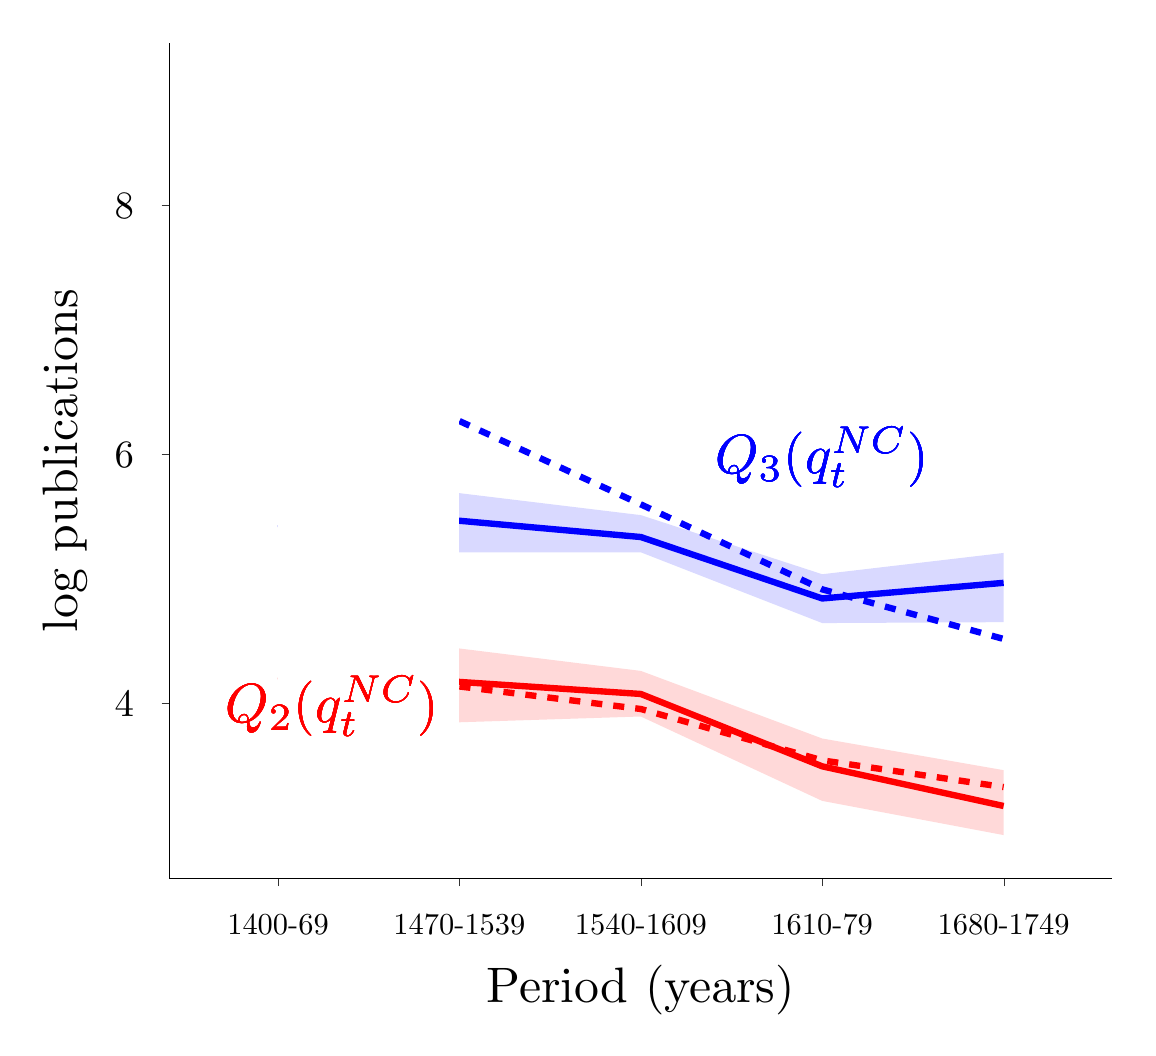
\begin{tikzpicture}[x=1pt,y=1pt]
\definecolor{fillColor}{RGB}{255,255,255}
\path[use as bounding box,fill=fillColor,fill opacity=0.00] (0,0) rectangle (397.48,361.35);
\begin{scope}
\path[clip] (  0.00,  0.00) rectangle (397.48,361.35);
\definecolor{drawColor}{RGB}{255,255,255}
\definecolor{fillColor}{RGB}{255,255,255}

\path[draw=drawColor,line width= 0.1pt,line join=round,line cap=round,fill=fillColor] (  0.00,  0.00) rectangle (397.48,361.35);
\end{scope}
\begin{scope}
\path[clip] ( 51.14, 53.86) rectangle (391.98,355.85);
\definecolor{fillColor}{RGB}{255,255,255}

\path[fill=fillColor] ( 51.14, 53.86) rectangle (391.98,355.85);
\definecolor{fillColor}{RGB}{255,0,0}

\path[fill=fillColor,fill opacity=0.15] ( 90.47,136.22) --
	(156.02,137.02) --
	(221.56,128.92) --
	(287.11,104.49) --
	(352.66, 93.05) --
	(352.66, 69.59) --
	(287.11, 81.94) --
	(221.56,112.44) --
	(156.02,110.35) --
	( 90.47,106.78) --
	cycle;

\path[] ( 90.47,136.22) --
	(156.02,137.02) --
	(221.56,128.92) --
	(287.11,104.49) --
	(352.66, 93.05);

\path[] (352.66, 69.59) --
	(287.11, 81.94) --
	(221.56,112.44) --
	(156.02,110.35) --
	( 90.47,106.78);
\definecolor{drawColor}{RGB}{255,0,0}

\path[draw=drawColor,line width= 2.3pt,line join=round] ( 90.47,126.97) --
	(156.02,124.94) --
	(221.56,120.58) --
	(287.11, 94.43) --
	(352.66, 80.10);

\path[draw=drawColor,line width= 2.3pt,dash pattern=on 4pt off 4pt ,line join=round] (156.02,123.30) --
	(221.56,115.15) --
	(287.11, 96.59) --
	(352.66, 86.95);
\definecolor{fillColor}{RGB}{0,0,255}

\path[fill=fillColor,fill opacity=0.15] ( 90.47,199.10) --
	(156.02,193.15) --
	(221.56,185.21) --
	(287.11,163.85) --
	(352.66,171.54) --
	(352.66,146.53) --
	(287.11,146.20) --
	(221.56,171.77) --
	(156.02,171.76) --
	( 90.47,164.34) --
	cycle;

\path[] ( 90.47,199.10) --
	(156.02,193.15) --
	(221.56,185.21) --
	(287.11,163.85) --
	(352.66,171.54);

\path[] (352.66,146.53) --
	(287.11,146.20) --
	(221.56,171.77) --
	(156.02,171.76) --
	( 90.47,164.34);
\definecolor{drawColor}{RGB}{0,0,255}

\path[draw=drawColor,line width= 2.3pt,line join=round] ( 90.47,180.48) --
	(156.02,183.17) --
	(221.56,177.29) --
	(287.11,155.09) --
	(352.66,160.74);

\path[draw=drawColor,line width= 2.3pt,dash pattern=on 4pt off 4pt ,line join=round] (156.02,219.20) --
	(221.56,189.09) --
	(287.11,158.39) --
	(352.66,140.46);
\definecolor{fillColor}{RGB}{255,255,255}

\path[fill=fillColor] ( 90.47, 53.86) rectangle (156.02,355.85);

\path[fill=fillColor] ( 90.47, 53.86) rectangle (156.02,355.85);

\path[fill=fillColor] ( 90.47, 53.86) rectangle (156.02,355.85);

\path[fill=fillColor] ( 90.47, 53.86) rectangle (156.02,355.85);

\path[fill=fillColor] ( 90.47, 53.86) rectangle (156.02,355.85);

\node[text=drawColor,anchor=base,inner sep=0pt, outer sep=0pt, scale=  1.99] at (287.11,200.25) {$Q_3(q_t^{NC})$};

\node[text=drawColor,anchor=base,inner sep=0pt, outer sep=0pt, scale=  1.99] at (287.11,200.25) {$Q_3(q_t^{NC})$};

\node[text=drawColor,anchor=base,inner sep=0pt, outer sep=0pt, scale=  1.99] at (287.11,200.25) {$Q_3(q_t^{NC})$};

\node[text=drawColor,anchor=base,inner sep=0pt, outer sep=0pt, scale=  1.99] at (287.11,200.25) {$Q_3(q_t^{NC})$};

\node[text=drawColor,anchor=base,inner sep=0pt, outer sep=0pt, scale=  1.99] at (287.11,200.25) {$Q_3(q_t^{NC})$};
\definecolor{drawColor}{RGB}{255,0,0}

\node[text=drawColor,anchor=base,inner sep=0pt, outer sep=0pt, scale=  1.99] at (110.14,110.23) {$Q_2(q_t^{NC})$};

\node[text=drawColor,anchor=base,inner sep=0pt, outer sep=0pt, scale=  1.99] at (110.14,110.23) {$Q_2(q_t^{NC})$};

\node[text=drawColor,anchor=base,inner sep=0pt, outer sep=0pt, scale=  1.99] at (110.14,110.23) {$Q_2(q_t^{NC})$};

\node[text=drawColor,anchor=base,inner sep=0pt, outer sep=0pt, scale=  1.99] at (110.14,110.23) {$Q_2(q_t^{NC})$};

\node[text=drawColor,anchor=base,inner sep=0pt, outer sep=0pt, scale=  1.99] at (110.14,110.23) {$Q_2(q_t^{NC})$};
\end{scope}
\begin{scope}
\path[clip] (  0.00,  0.00) rectangle (397.48,361.35);
\definecolor{drawColor}{RGB}{0,0,0}

\path[draw=drawColor,line width= 0.1pt,line join=round] ( 51.14, 53.86) --
	( 51.14,355.85);
\end{scope}
\begin{scope}
\path[clip] (  0.00,  0.00) rectangle (397.48,361.35);
\definecolor{drawColor}{RGB}{0,0,0}

\node[text=drawColor,anchor=base east,inner sep=0pt, outer sep=0pt, scale=  1.40] at ( 38.39,112.27) {4};

\node[text=drawColor,anchor=base east,inner sep=0pt, outer sep=0pt, scale=  1.40] at ( 38.39,202.28) {6};

\node[text=drawColor,anchor=base east,inner sep=0pt, outer sep=0pt, scale=  1.40] at ( 38.39,292.30) {8};
\end{scope}
\begin{scope}
\path[clip] (  0.00,  0.00) rectangle (397.48,361.35);
\definecolor{drawColor}{gray}{0.20}

\path[draw=drawColor,line width= 0.1pt,line join=round] ( 48.39,117.09) --
	( 51.14,117.09);

\path[draw=drawColor,line width= 0.1pt,line join=round] ( 48.39,207.11) --
	( 51.14,207.11);

\path[draw=drawColor,line width= 0.1pt,line join=round] ( 48.39,297.12) --
	( 51.14,297.12);
\end{scope}
\begin{scope}
\path[clip] (  0.00,  0.00) rectangle (397.48,361.35);
\definecolor{drawColor}{RGB}{0,0,0}

\path[draw=drawColor,line width= 0.1pt,line join=round] ( 51.14, 53.86) --
	(391.98, 53.86);
\end{scope}
\begin{scope}
\path[clip] (  0.00,  0.00) rectangle (397.48,361.35);
\definecolor{drawColor}{gray}{0.20}

\path[draw=drawColor,line width= 0.1pt,line join=round] ( 90.47, 51.11) --
	( 90.47, 53.86);

\path[draw=drawColor,line width= 0.1pt,line join=round] (156.02, 51.11) --
	(156.02, 53.86);

\path[draw=drawColor,line width= 0.1pt,line join=round] (221.56, 51.11) --
	(221.56, 53.86);

\path[draw=drawColor,line width= 0.1pt,line join=round] (287.11, 51.11) --
	(287.11, 53.86);

\path[draw=drawColor,line width= 0.1pt,line join=round] (352.66, 51.11) --
	(352.66, 53.86);
\end{scope}
\begin{scope}
\path[clip] (  0.00,  0.00) rectangle (397.48,361.35);
\definecolor{drawColor}{RGB}{0,0,0}

\node[text=drawColor,anchor=base,inner sep=0pt, outer sep=0pt, scale=  1.10] at ( 90.47, 33.53) {1400-69};

\node[text=drawColor,anchor=base,inner sep=0pt, outer sep=0pt, scale=  1.10] at (156.02, 33.53) {1470-1539};

\node[text=drawColor,anchor=base,inner sep=0pt, outer sep=0pt, scale=  1.10] at (221.56, 33.53) {1540-1609};

\node[text=drawColor,anchor=base,inner sep=0pt, outer sep=0pt, scale=  1.10] at (287.11, 33.53) {1610-79};

\node[text=drawColor,anchor=base,inner sep=0pt, outer sep=0pt, scale=  1.10] at (352.66, 33.53) {1680-1749};
\end{scope}
\begin{scope}
\path[clip] (  0.00,  0.00) rectangle (397.48,361.35);
\definecolor{drawColor}{RGB}{0,0,0}

\node[text=drawColor,anchor=base,inner sep=0pt, outer sep=0pt, scale=  1.80] at (221.56,  9.00) {Period (years)};
\end{scope}
\begin{scope}
\path[clip] (  0.00,  0.00) rectangle (397.48,361.35);
\definecolor{drawColor}{RGB}{0,0,0}

\node[text=drawColor,rotate= 90.00,anchor=base,inner sep=0pt, outer sep=0pt, scale=  1.80] at ( 17.90,204.86) {log publications};
\end{scope}
\end{tikzpicture}
}
}
	\caption{Model fit (upper panels), over-identification checks (lower panels).\\ Data (solid) and simulations (dashed).}
	\label{fig:fit}
\end{figure}

%Note that our parameter estimates would be biased if the convergence forces, which imply larger growth rates for lower levels of knowledge, were not correctly taken into account by the model. In Appendix~\ref{O-app:robust-convergence} we show that the model matches well the publication dynamics of Great Britain, which lagged behind Italy in the fifteenth century.
%\section{The Decline of Italy and Convergence} \label{app:robust-convergence}
%In this paper we use a structural model to assess quantitatively the role of censorship in the decline in total publications per scholar in Italy. The credibility of our quantification depends on whether the convergence forces, which imply larger growth rates for lower levels of knowledge, are correctly taken into account by the model. If this was not the case, our parameter estimates would be biased.
%For example, if the model convergence forces were stronger than the actual ones, the estimated effect of censorship would be too large because of the need to keep the level of publications in Italy low

The model fit is reported in Figure~\ref{fig:fit}, upper panels. The simulated variables rarely lie outside the $95\%$ confidence interval of the data moments. %An exception is the $75^{th}$ percentile of the overall knowledge quality. This reflects that the underlying empirical distribution does not follow exactly a Fr\'echet distribution like in the model.

%As a test of the theory, we compare our results to empirical observations that were not used to identify the parameters. Looking at the quality of censored $q_t^R$ and non-censored authors $q_t^{NC}$ (Figure~\ref{fig:fit}, lower panels) is particularly interesting as it allows us to test whether printers choose their sector according to its (relative) quality.\footnote{The distribution of quality of censored and revolutionary authors is the same because censorship is random. The distribution of quality of non-censored authors  $q_t^{NC}$ is obtained by drawing from the distribution of $q^R_t$ with probability $p^{nc}$ and from the distribution of $q^C_t$ with probability $1-p^{nc}$, where $p^{nc}$ is the share of \textit{printed} books that are revolutionary.}  This mechanism is summarized by Equation (\ref{eq:sharer2}): the share of revolutionary authors can assume one and only one variable given the ratio of the quality in the two sectors. This ratio can be proxied by the ratio of censored to non-censored authors' quality, which we can measure in the data. Since the model fit well the dynamics of censored and non-censored authors, we can assert that Equation~(\ref{eq:sharer2}) is likely to hold in the data too. The model also predicts that the share of revolutionary ideas was increasing before $t=3$. This is consistent with the fact that the share of censored books was larger in the period 1470-1539 than 1400-1469. Moreover, the average difference in quality between censored and non-censored authors decreases from 3.60 in 1470-1539 to 1.46 in 1680-1749.

As a test of the theory, we compare our results to empirical observations that were not used to identify the parameters. Looking at the quality of censored $q_t^R$ and non-censored authors $q_t^{NC}$ (Figure~\ref{fig:fit}, lower panels) is particularly interesting.\footnote{The distribution of quality of censored and revolutionary authors is the same because censorship is random. The distribution of quality of non-censored authors  $q_t^{NC}$ is obtained by drawing from the distribution of $q^R_t$ with probability $p^{nc}$ and from the distribution of $q^C_t$ with probability $1-p^{nc}$, where $p^{nc}$ is the share of \textit{printed} books that are revolutionary.} This is because from the model's theoretical restrictions it follows that the observed share of censored authors and overall quality imply specific distributions of $q_t^R$ and $q_t^{NC}$ for a given parametrization.\footnote{Equation (\ref{eq:sharer2}) implies that the share of revolutionary authors can assume one and only one value given the ratio of quality in the two sectors $k^R_t$ and $k^C_t$. Since authors’ quality  in sector $j$ is strictly increasing in $k^j_t$, a given level of overall quality and share of censored authors can only be generated by two specific values of $k^R_t$ and $k^C_t$ for a specific parametrization. Finally, note that $k^R_t$ and $k^C_t$ are the model state variables: their value implies a specific quality of censored and non-censored authors.} Without targeting these moments in particular, the model matches them well, which gives credence to the model's mechanisms. The model also predicts that the share of revolutionary ideas was increasing before $t=3$. This is consistent with the fact that the share of censored books was larger in the period 1470-1539 than 1400-1469. Moreover, the average difference in quality between censored and non-censored authors decreases from 2.91 in 1470-1539 to 1.72 in 1680-1749.

As a second out of sample test of our theory, we compare the dynamics of publications in Great Britain with model simulations. Data for Great Britain are in Appendix~\ref{O-app:british}. We simulate the dynamics of publications by decreasing the initial conditions in the state of knowledge ($k^R_1,k^C_1$) used for Italy by $45\%$ to match the median number of log publications in Great Britain in $t=2$.\footnote{We consider $t=2$ and not $t=1$ because we have less than 20 published scholars for $t=1$.} The remaining parameters are set equal to those used for Italy, except for $\overline{\beta}$, which is set to 0 (no censorship). We also recompute the process for $\mu_t$ using GDP per capita. The results are shown in Figure~\ref{fig:Sq_uk}.


%UPDATED 29 AUG 2022=========================================================================================================================
\begin{figure}[htb]	
	\centering
	\hspace*{-1cm}
	
	% include second image
	\scalebox{0.36}{% Created by tikzDevice version 0.12.3.1 on 2022-09-19 22:27:57
% !TEX encoding = UTF-8 Unicode
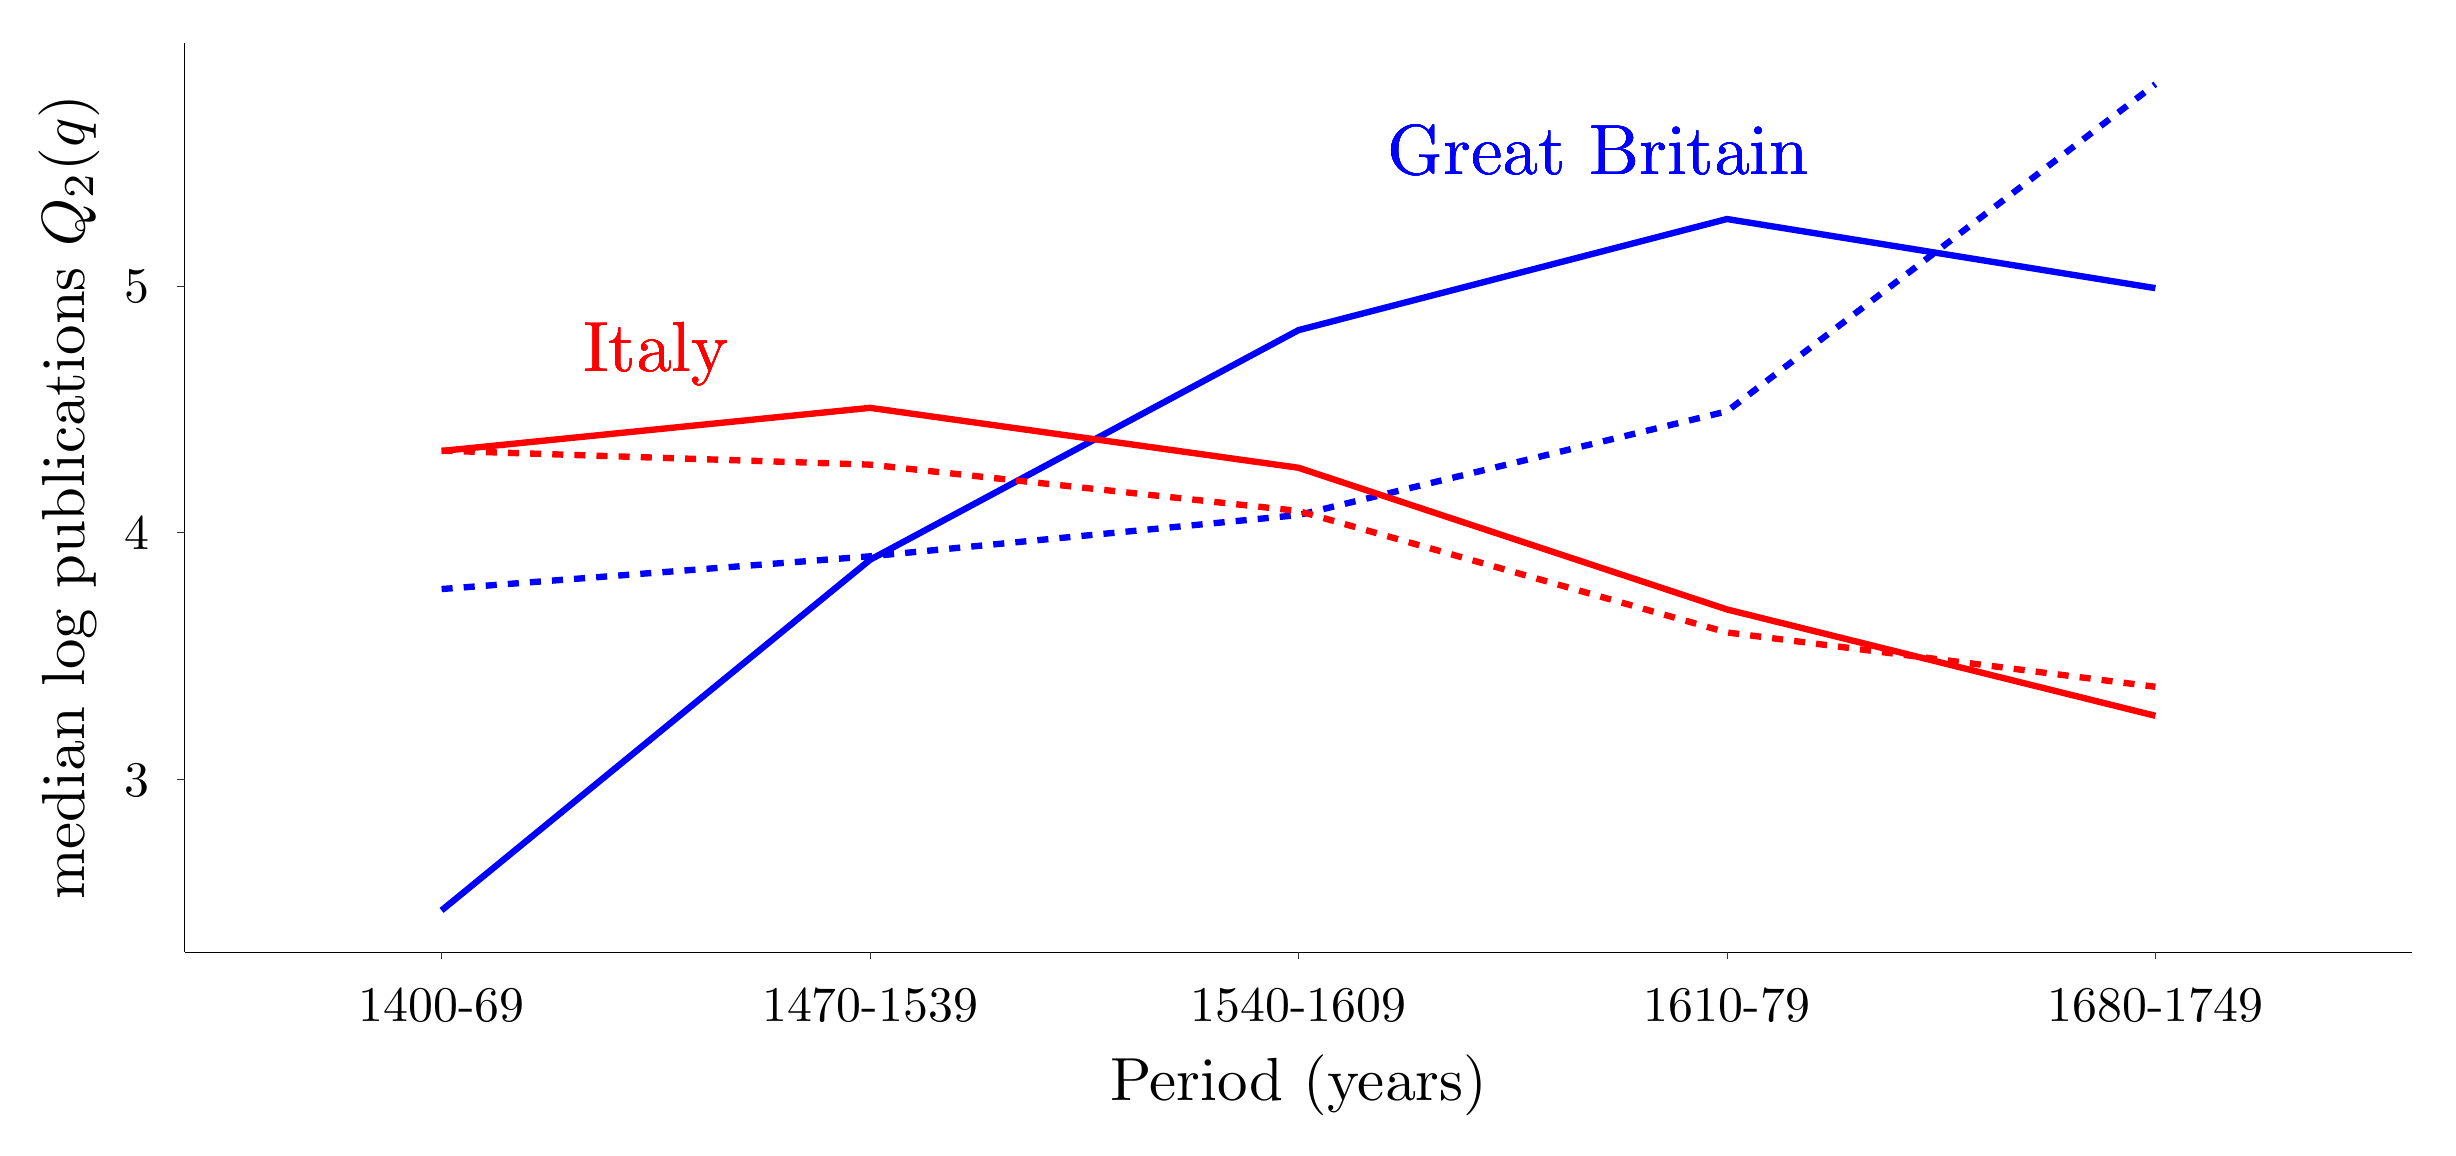
\begin{tikzpicture}[x=1pt,y=1pt]
\definecolor{fillColor}{RGB}{255,255,255}
\path[use as bounding box,fill=fillColor,fill opacity=0.00] (0,0) rectangle (867.24,397.48);
\begin{scope}
\path[clip] (  0.00,  0.00) rectangle (867.24,397.48);
\definecolor{drawColor}{RGB}{255,255,255}
\definecolor{fillColor}{RGB}{255,255,255}

\path[draw=drawColor,line width= 0.1pt,line join=round,line cap=round,fill=fillColor] (  0.00,  0.00) rectangle (867.24,397.48);
\end{scope}
\begin{scope}
\path[clip] ( 56.68, 63.57) rectangle (861.74,391.98);
\definecolor{fillColor}{RGB}{255,255,255}

\path[fill=fillColor] ( 56.68, 63.57) rectangle (861.74,391.98);
\definecolor{drawColor}{RGB}{0,0,255}

\path[draw=drawColor,line width= 2.3pt,line join=round] (149.57, 78.50) --
	(304.39,205.20) --
	(459.21,288.18) --
	(614.03,328.33) --
	(768.85,303.35);

\path[draw=drawColor,line width= 2.3pt,dash pattern=on 4pt off 4pt ,line join=round] (149.57,194.62) --
	(304.39,206.45) --
	(459.21,221.36) --
	(614.03,258.84) --
	(768.85,377.06);
\definecolor{drawColor}{RGB}{255,0,0}

\path[draw=drawColor,line width= 2.3pt,line join=round] (149.57,244.52) --
	(304.39,260.10) --
	(459.21,238.45) --
	(614.03,187.26) --
	(768.85,148.82);

\path[draw=drawColor,line width= 2.3pt,dash pattern=on 4pt off 4pt ,line join=round] (149.57,244.63) --
	(304.39,239.58) --
	(459.21,222.83) --
	(614.03,178.94) --
	(768.85,159.31);
\definecolor{drawColor}{RGB}{0,0,255}

\node[text=drawColor,anchor=base,inner sep=0pt, outer sep=0pt, scale=  2.56] at (567.58,344.49) {Great Britain};

\node[text=drawColor,anchor=base,inner sep=0pt, outer sep=0pt, scale=  2.56] at (567.58,344.49) {Great Britain};

\node[text=drawColor,anchor=base,inner sep=0pt, outer sep=0pt, scale=  2.56] at (567.58,344.49) {Great Britain};

\node[text=drawColor,anchor=base,inner sep=0pt, outer sep=0pt, scale=  2.56] at (567.58,344.49) {Great Britain};

\node[text=drawColor,anchor=base,inner sep=0pt, outer sep=0pt, scale=  2.56] at (567.58,344.49) {Great Britain};
\definecolor{drawColor}{RGB}{255,0,0}

\node[text=drawColor,anchor=base,inner sep=0pt, outer sep=0pt, scale=  2.56] at (226.98,273.12) {Italy};

\node[text=drawColor,anchor=base,inner sep=0pt, outer sep=0pt, scale=  2.56] at (226.98,273.12) {Italy};

\node[text=drawColor,anchor=base,inner sep=0pt, outer sep=0pt, scale=  2.56] at (226.98,273.12) {Italy};

\node[text=drawColor,anchor=base,inner sep=0pt, outer sep=0pt, scale=  2.56] at (226.98,273.12) {Italy};

\node[text=drawColor,anchor=base,inner sep=0pt, outer sep=0pt, scale=  2.56] at (226.98,273.12) {Italy};
\end{scope}
\begin{scope}
\path[clip] (  0.00,  0.00) rectangle (867.24,397.48);
\definecolor{drawColor}{RGB}{0,0,0}

\path[draw=drawColor,line width= 0.1pt,line join=round] ( 56.68, 63.57) --
	( 56.68,391.98);
\end{scope}
\begin{scope}
\path[clip] (  0.00,  0.00) rectangle (867.24,397.48);
\definecolor{drawColor}{RGB}{0,0,0}

\node[text=drawColor,anchor=base east,inner sep=0pt, outer sep=0pt, scale=  1.80] at ( 43.93,119.59) {3};

\node[text=drawColor,anchor=base east,inner sep=0pt, outer sep=0pt, scale=  1.80] at ( 43.93,208.82) {4};

\node[text=drawColor,anchor=base east,inner sep=0pt, outer sep=0pt, scale=  1.80] at ( 43.93,298.04) {5};
\end{scope}
\begin{scope}
\path[clip] (  0.00,  0.00) rectangle (867.24,397.48);
\definecolor{drawColor}{gray}{0.20}

\path[draw=drawColor,line width= 0.1pt,line join=round] ( 53.93,125.79) --
	( 56.68,125.79);

\path[draw=drawColor,line width= 0.1pt,line join=round] ( 53.93,215.02) --
	( 56.68,215.02);

\path[draw=drawColor,line width= 0.1pt,line join=round] ( 53.93,304.24) --
	( 56.68,304.24);
\end{scope}
\begin{scope}
\path[clip] (  0.00,  0.00) rectangle (867.24,397.48);
\definecolor{drawColor}{RGB}{0,0,0}

\path[draw=drawColor,line width= 0.1pt,line join=round] ( 56.68, 63.57) --
	(861.74, 63.57);
\end{scope}
\begin{scope}
\path[clip] (  0.00,  0.00) rectangle (867.24,397.48);
\definecolor{drawColor}{gray}{0.20}

\path[draw=drawColor,line width= 0.1pt,line join=round] (149.57, 60.82) --
	(149.57, 63.57);

\path[draw=drawColor,line width= 0.1pt,line join=round] (304.39, 60.82) --
	(304.39, 63.57);

\path[draw=drawColor,line width= 0.1pt,line join=round] (459.21, 60.82) --
	(459.21, 63.57);

\path[draw=drawColor,line width= 0.1pt,line join=round] (614.03, 60.82) --
	(614.03, 63.57);

\path[draw=drawColor,line width= 0.1pt,line join=round] (768.85, 60.82) --
	(768.85, 63.57);
\end{scope}
\begin{scope}
\path[clip] (  0.00,  0.00) rectangle (867.24,397.48);
\definecolor{drawColor}{RGB}{0,0,0}

\node[text=drawColor,anchor=base,inner sep=0pt, outer sep=0pt, scale=  1.80] at (149.57, 38.43) {1400-69};

\node[text=drawColor,anchor=base,inner sep=0pt, outer sep=0pt, scale=  1.80] at (304.39, 38.43) {1470-1539};

\node[text=drawColor,anchor=base,inner sep=0pt, outer sep=0pt, scale=  1.80] at (459.21, 38.43) {1540-1609};

\node[text=drawColor,anchor=base,inner sep=0pt, outer sep=0pt, scale=  1.80] at (614.03, 38.43) {1610-79};

\node[text=drawColor,anchor=base,inner sep=0pt, outer sep=0pt, scale=  1.80] at (768.85, 38.43) {1680-1749};
\end{scope}
\begin{scope}
\path[clip] (  0.00,  0.00) rectangle (867.24,397.48);
\definecolor{drawColor}{RGB}{0,0,0}

\node[text=drawColor,anchor=base,inner sep=0pt, outer sep=0pt, scale=  2.20] at (459.21,  9.78) {Period (years)};
\end{scope}
\begin{scope}
\path[clip] (  0.00,  0.00) rectangle (867.24,397.48);
\definecolor{drawColor}{RGB}{0,0,0}

\node[text=drawColor,rotate= 90.00,anchor=base,inner sep=0pt, outer sep=0pt, scale=  2.20] at ( 20.65,227.78) {median log publications  $Q_2(q)$};
\end{scope}
\end{tikzpicture}
e (  1.58);
\definecolor{drawColor}{RGB}{0,0,0}

\node[text=drawColor,anchor=base west,inner sep=0pt, outer sep=0pt, scale=  1.00] at (789.19, 99.50) {Best};

\node[text=drawColor,anchor=base west,inner sep=0pt, outer sep=0pt, scale=  1.00] at (789.19, 87.50) {Mean};

\node[text=drawColor,anchor=base west,inner sep=0pt, outer sep=0pt, scale=  1.00] at (789.19, 75.50) {Median};
\end{scope}
\end{tikzpicture}
 }
	
	\caption{Median scholars quality $Q_2(q_t)$. Blue: Great Britain. Red: Italy.  \\ Data (solid) and simulations (dashed). }
	\label{fig:Sq_uk}
\end{figure}

Simulations of median log publications in Great Britain are relatively close to their data counterpart, despite we did not used them in the estimation procedure. The model shows the ability to match well the British data when the initial conditions are set to a level lower than the Italian case. This result supports the claim that the model predicts correctly the catching up and overtaking of Great Britain, through a mix of convergence forces acting in the dynamics of $m_t$, differences in the  exogenous process of $\mu_t$, and the presence of censorship in Italy.


\subsubsection*{The Role of Censorship in Knowledge Formation}

What is the role of the Catholic Church in the demise in knowledge production in early modern Italy? How much of this effect is driven by selection into the revolutionary/compliant sectors? In this section we answer these questions by comparing model simulations with and without censorship. This is done by setting the rate of censorship $\overline{\beta}$ to $0$ in the no-censorship scenario. Figure~\ref{fig:exp} illustrates the outcomes of the experiments.

%%%%%%%%%%%%%%%%%%%%%%%%%%%%%%%%%%%%%%
%Const. exp.  1
%%%%%%%%%%%%%%%%%%%%%%%%%%%%%%%%%%%%%%
%UPDATED 29 AUG 2022=========================================================================================================================
\begin{figure}[htb]	
	\centering
	\hspace*{-1cm}
	\begin{subfigure}{.49\textwidth}
		\centering
		% include first image
		\caption{Share of revolutionary scholars ($m_t$)\\\textcolor{white}{a}}
		\label{sf:ra}
		\scalebox{0.55}{% Created by tikzDevice version 0.12.3.1 on 2022-09-19 22:27:55
% !TEX encoding = UTF-8 Unicode
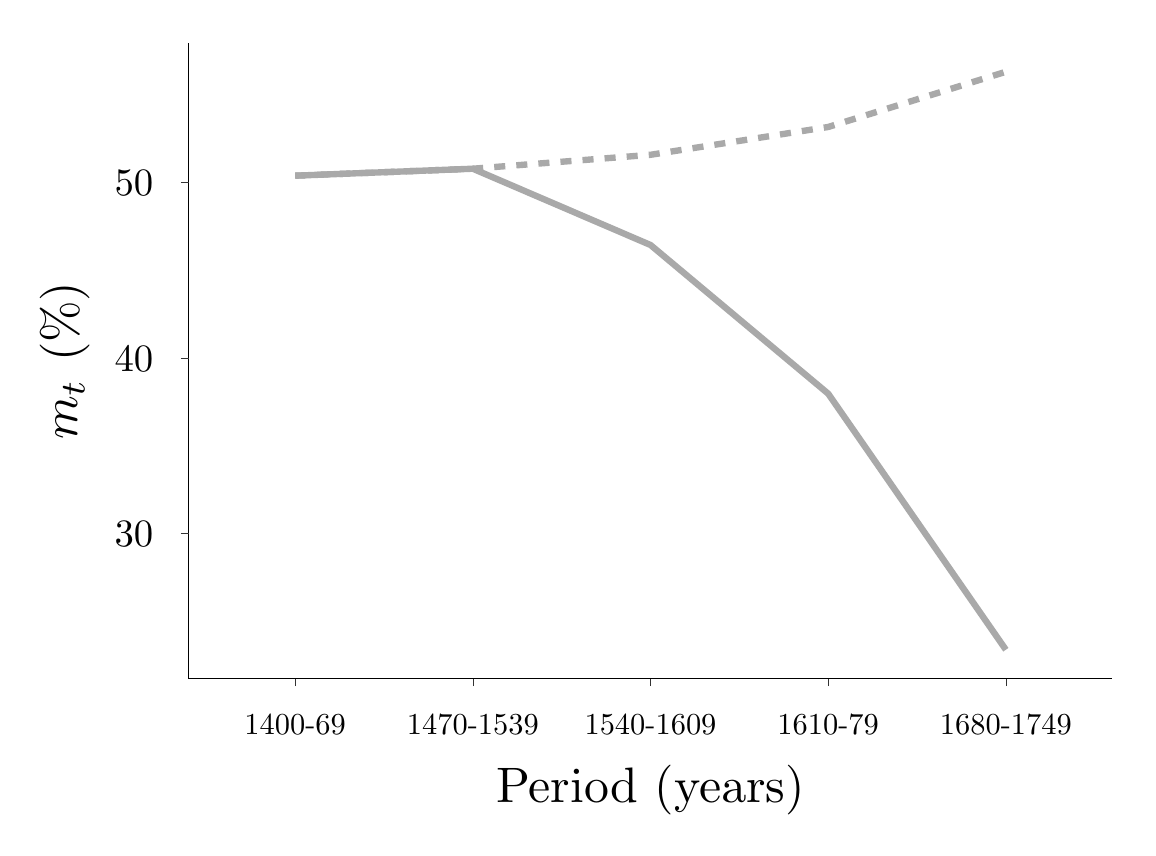
\begin{tikzpicture}[x=1pt,y=1pt]
\definecolor{fillColor}{RGB}{255,255,255}
\path[use as bounding box,fill=fillColor,fill opacity=0.00] (0,0) rectangle (397.48,289.08);
\begin{scope}
\path[clip] (  0.00,  0.00) rectangle (397.48,289.08);
\definecolor{drawColor}{RGB}{255,255,255}
\definecolor{fillColor}{RGB}{255,255,255}

\path[draw=drawColor,line width= 0.1pt,line join=round,line cap=round,fill=fillColor] (  0.00,  0.00) rectangle (397.48,289.08);
\end{scope}
\begin{scope}
\path[clip] ( 58.14, 53.86) rectangle (391.98,283.58);
\definecolor{fillColor}{RGB}{255,255,255}

\path[fill=fillColor] ( 58.14, 53.86) rectangle (391.98,283.58);
\definecolor{drawColor}{RGB}{169,169,169}

\path[draw=drawColor,line width= 2.3pt,line join=round] ( 96.66,235.59) --
	(160.86,238.11) --
	(225.06,210.55) --
	(289.26,156.83) --
	(353.46, 64.30);

\path[draw=drawColor,line width= 2.3pt,dash pattern=on 4pt off 4pt ,line join=round] ( 96.66,235.59) --
	(160.86,238.11) --
	(225.06,243.14) --
	(289.26,253.19) --
	(353.46,273.14);
\end{scope}
\begin{scope}
\path[clip] (  0.00,  0.00) rectangle (397.48,289.08);
\definecolor{drawColor}{RGB}{0,0,0}

\path[draw=drawColor,line width= 0.1pt,line join=round] ( 58.14, 53.86) --
	( 58.14,283.58);
\end{scope}
\begin{scope}
\path[clip] (  0.00,  0.00) rectangle (397.48,289.08);
\definecolor{drawColor}{RGB}{0,0,0}

\node[text=drawColor,anchor=base east,inner sep=0pt, outer sep=0pt, scale=  1.40] at ( 45.39,101.57) {30};

\node[text=drawColor,anchor=base east,inner sep=0pt, outer sep=0pt, scale=  1.40] at ( 45.39,164.91) {40};

\node[text=drawColor,anchor=base east,inner sep=0pt, outer sep=0pt, scale=  1.40] at ( 45.39,228.26) {50};
\end{scope}
\begin{scope}
\path[clip] (  0.00,  0.00) rectangle (397.48,289.08);
\definecolor{drawColor}{gray}{0.20}

\path[draw=drawColor,line width= 0.1pt,line join=round] ( 55.39,106.39) --
	( 58.14,106.39);

\path[draw=drawColor,line width= 0.1pt,line join=round] ( 55.39,169.73) --
	( 58.14,169.73);

\path[draw=drawColor,line width= 0.1pt,line join=round] ( 55.39,233.08) --
	( 58.14,233.08);
\end{scope}
\begin{scope}
\path[clip] (  0.00,  0.00) rectangle (397.48,289.08);
\definecolor{drawColor}{RGB}{0,0,0}

\path[draw=drawColor,line width= 0.1pt,line join=round] ( 58.14, 53.86) --
	(391.98, 53.86);
\end{scope}
\begin{scope}
\path[clip] (  0.00,  0.00) rectangle (397.48,289.08);
\definecolor{drawColor}{gray}{0.20}

\path[draw=drawColor,line width= 0.1pt,line join=round] ( 96.66, 51.11) --
	( 96.66, 53.86);

\path[draw=drawColor,line width= 0.1pt,line join=round] (160.86, 51.11) --
	(160.86, 53.86);

\path[draw=drawColor,line width= 0.1pt,line join=round] (225.06, 51.11) --
	(225.06, 53.86);

\path[draw=drawColor,line width= 0.1pt,line join=round] (289.26, 51.11) --
	(289.26, 53.86);

\path[draw=drawColor,line width= 0.1pt,line join=round] (353.46, 51.11) --
	(353.46, 53.86);
\end{scope}
\begin{scope}
\path[clip] (  0.00,  0.00) rectangle (397.48,289.08);
\definecolor{drawColor}{RGB}{0,0,0}

\node[text=drawColor,anchor=base,inner sep=0pt, outer sep=0pt, scale=  1.10] at ( 96.66, 33.53) {1400-69};

\node[text=drawColor,anchor=base,inner sep=0pt, outer sep=0pt, scale=  1.10] at (160.86, 33.53) {1470-1539};

\node[text=drawColor,anchor=base,inner sep=0pt, outer sep=0pt, scale=  1.10] at (225.06, 33.53) {1540-1609};

\node[text=drawColor,anchor=base,inner sep=0pt, outer sep=0pt, scale=  1.10] at (289.26, 33.53) {1610-79};

\node[text=drawColor,anchor=base,inner sep=0pt, outer sep=0pt, scale=  1.10] at (353.46, 33.53) {1680-1749};
\end{scope}
\begin{scope}
\path[clip] (  0.00,  0.00) rectangle (397.48,289.08);
\definecolor{drawColor}{RGB}{0,0,0}

\node[text=drawColor,anchor=base,inner sep=0pt, outer sep=0pt, scale=  1.80] at (225.06,  9.00) {Period (years)};
\end{scope}
\begin{scope}
\path[clip] (  0.00,  0.00) rectangle (397.48,289.08);
\definecolor{drawColor}{RGB}{0,0,0}

\node[text=drawColor,rotate= 90.00,anchor=base,inner sep=0pt, outer sep=0pt, scale=  1.80] at ( 17.90,168.72) {$m_t$ (\%)};
\end{scope}
\end{tikzpicture}
 }
	\end{subfigure}\hspace{-5mm}
	\begin{subfigure}{.49\textwidth}
		\centering
		% include second image
		\caption{\textcolor{blue}{Overall}, \textcolor{red}{revolutionary}\\ \textcolor{orange}{compliant} scholars quality}
		\label{sf:dq}
		\scalebox{0.55}{% Created by tikzDevice version 0.12.3.1 on 2022-09-19 22:27:55
% !TEX encoding = UTF-8 Unicode
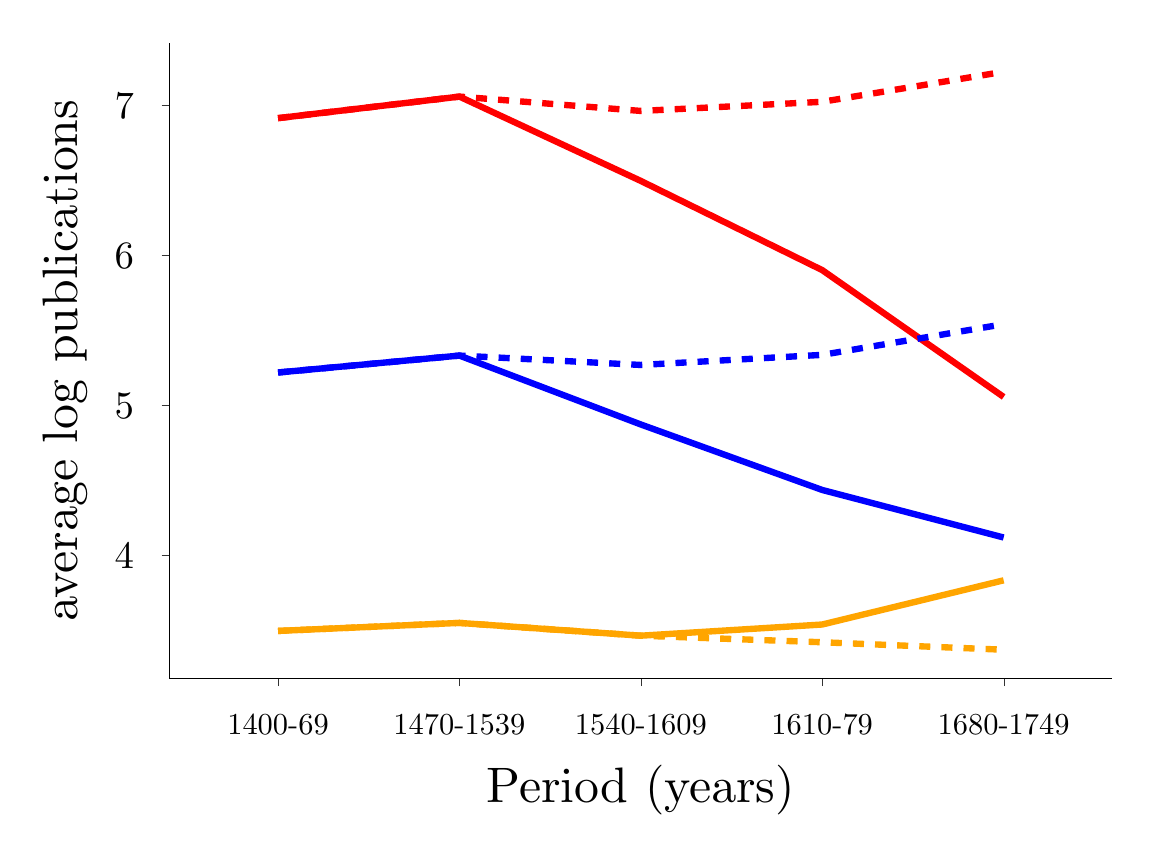
\begin{tikzpicture}[x=1pt,y=1pt]
\definecolor{fillColor}{RGB}{255,255,255}
\path[use as bounding box,fill=fillColor,fill opacity=0.00] (0,0) rectangle (397.48,289.08);
\begin{scope}
\path[clip] (  0.00,  0.00) rectangle (397.48,289.08);
\definecolor{drawColor}{RGB}{255,255,255}
\definecolor{fillColor}{RGB}{255,255,255}

\path[draw=drawColor,line width= 0.1pt,line join=round,line cap=round,fill=fillColor] (  0.00,  0.00) rectangle (397.48,289.08);
\end{scope}
\begin{scope}
\path[clip] ( 51.14, 53.86) rectangle (391.98,283.58);
\definecolor{fillColor}{RGB}{255,255,255}

\path[fill=fillColor] ( 51.14, 53.86) rectangle (391.98,283.58);
\definecolor{drawColor}{RGB}{255,0,0}

\path[draw=drawColor,line width= 2.3pt,line join=round] ( 90.47,256.38) --
	(156.02,264.17) --
	(221.56,233.70) --
	(287.11,201.47) --
	(352.66,155.64);

\path[draw=drawColor,line width= 2.3pt,dash pattern=on 4pt off 4pt ,line join=round] ( 90.47,256.38) --
	(156.02,264.17) --
	(221.56,258.99) --
	(287.11,262.29) --
	(352.66,273.14);
\definecolor{drawColor}{RGB}{0,0,255}

\path[draw=drawColor,line width= 2.3pt,line join=round] ( 90.47,164.47) --
	(156.02,170.59) --
	(221.56,145.69) --
	(287.11,122.03) --
	(352.66,104.85);

\path[draw=drawColor,line width= 2.3pt,dash pattern=on 4pt off 4pt ,line join=round] ( 90.47,164.47) --
	(156.02,170.59) --
	(221.56,167.20) --
	(287.11,170.85) --
	(352.66,181.93);
\definecolor{drawColor}{RGB}{255,165,0}

\path[draw=drawColor,line width= 2.3pt,line join=round] ( 90.47, 71.09) --
	(156.02, 73.99) --
	(221.56, 69.37) --
	(287.11, 73.41) --
	(352.66, 89.38);

\path[draw=drawColor,line width= 2.3pt,dash pattern=on 4pt off 4pt ,line join=round] ( 90.47, 71.09) --
	(156.02, 73.99) --
	(221.56, 69.37) --
	(287.11, 67.00) --
	(352.66, 64.30);
\end{scope}
\begin{scope}
\path[clip] (  0.00,  0.00) rectangle (397.48,289.08);
\definecolor{drawColor}{RGB}{0,0,0}

\path[draw=drawColor,line width= 0.1pt,line join=round] ( 51.14, 53.86) --
	( 51.14,283.58);
\end{scope}
\begin{scope}
\path[clip] (  0.00,  0.00) rectangle (397.48,289.08);
\definecolor{drawColor}{RGB}{0,0,0}

\node[text=drawColor,anchor=base east,inner sep=0pt, outer sep=0pt, scale=  1.40] at ( 38.39, 93.70) {4};

\node[text=drawColor,anchor=base east,inner sep=0pt, outer sep=0pt, scale=  1.40] at ( 38.39,147.89) {5};

\node[text=drawColor,anchor=base east,inner sep=0pt, outer sep=0pt, scale=  1.40] at ( 38.39,202.08) {6};

\node[text=drawColor,anchor=base east,inner sep=0pt, outer sep=0pt, scale=  1.40] at ( 38.39,256.27) {7};
\end{scope}
\begin{scope}
\path[clip] (  0.00,  0.00) rectangle (397.48,289.08);
\definecolor{drawColor}{gray}{0.20}

\path[draw=drawColor,line width= 0.1pt,line join=round] ( 48.39, 98.52) --
	( 51.14, 98.52);

\path[draw=drawColor,line width= 0.1pt,line join=round] ( 48.39,152.71) --
	( 51.14,152.71);

\path[draw=drawColor,line width= 0.1pt,line join=round] ( 48.39,206.90) --
	( 51.14,206.90);

\path[draw=drawColor,line width= 0.1pt,line join=round] ( 48.39,261.09) --
	( 51.14,261.09);
\end{scope}
\begin{scope}
\path[clip] (  0.00,  0.00) rectangle (397.48,289.08);
\definecolor{drawColor}{RGB}{0,0,0}

\path[draw=drawColor,line width= 0.1pt,line join=round] ( 51.14, 53.86) --
	(391.98, 53.86);
\end{scope}
\begin{scope}
\path[clip] (  0.00,  0.00) rectangle (397.48,289.08);
\definecolor{drawColor}{gray}{0.20}

\path[draw=drawColor,line width= 0.1pt,line join=round] ( 90.47, 51.11) --
	( 90.47, 53.86);

\path[draw=drawColor,line width= 0.1pt,line join=round] (156.02, 51.11) --
	(156.02, 53.86);

\path[draw=drawColor,line width= 0.1pt,line join=round] (221.56, 51.11) --
	(221.56, 53.86);

\path[draw=drawColor,line width= 0.1pt,line join=round] (287.11, 51.11) --
	(287.11, 53.86);

\path[draw=drawColor,line width= 0.1pt,line join=round] (352.66, 51.11) --
	(352.66, 53.86);
\end{scope}
\begin{scope}
\path[clip] (  0.00,  0.00) rectangle (397.48,289.08);
\definecolor{drawColor}{RGB}{0,0,0}

\node[text=drawColor,anchor=base,inner sep=0pt, outer sep=0pt, scale=  1.10] at ( 90.47, 33.53) {1400-69};

\node[text=drawColor,anchor=base,inner sep=0pt, outer sep=0pt, scale=  1.10] at (156.02, 33.53) {1470-1539};

\node[text=drawColor,anchor=base,inner sep=0pt, outer sep=0pt, scale=  1.10] at (221.56, 33.53) {1540-1609};

\node[text=drawColor,anchor=base,inner sep=0pt, outer sep=0pt, scale=  1.10] at (287.11, 33.53) {1610-79};

\node[text=drawColor,anchor=base,inner sep=0pt, outer sep=0pt, scale=  1.10] at (352.66, 33.53) {1680-1749};
\end{scope}
\begin{scope}
\path[clip] (  0.00,  0.00) rectangle (397.48,289.08);
\definecolor{drawColor}{RGB}{0,0,0}

\node[text=drawColor,anchor=base,inner sep=0pt, outer sep=0pt, scale=  1.80] at (221.56,  9.00) {Period (years)};
\end{scope}
\begin{scope}
\path[clip] (  0.00,  0.00) rectangle (397.48,289.08);
\definecolor{drawColor}{RGB}{0,0,0}

\node[text=drawColor,rotate= 90.00,anchor=base,inner sep=0pt, outer sep=0pt, scale=  1.80] at ( 17.90,168.72) {average log publications};
\end{scope}
\end{tikzpicture}
 }
	\end{subfigure}

	\caption{Baseline simulations (solid), simulations without censorship (dashed)}
	\label{fig:exp}
\end{figure}



Without censorship, the share or revolutionary authors $m_t$ would have kept increasing. It would have reached 56\% in $t=5$, instead of decreasing to 23\% in $t=5$. This fact demonstrates the effectiveness of censorship, which can change the dynamics of revolutionary ideas drastically. Moreover, censorship has the unintended effect of reducing the overall quality of scholars, which is 35\% lower under the baseline than in the $\overline{\beta}=0$ scenario.

\citeN{becker2021} analyze the effect of censorship on knowledge growth by establishing a empirical correlation between
 the number of famous people born in, or migrating into, a city and the number of indexed books printed in that city. Here we look at another, complementary, dimension by considering the actual publications of the scholars. Our structural approach also allows to quantify the effects, and to propose an interpretation of these effects, through the lens of our theory. Of course, in doing so, we impose more restrictions on the data than the reduced form approach of  \citeN{becker2021}  does.

The loss in  the overall quality is  driven both by a reduction in the stock of knowledge \textit{within each sector} and by self-selection \textit{across sectors}.   This result comes from the following decomposition:
\begin{multline}\label{eq:deco}
\underbrace{q_5-\hat{q}_5}_{\text{=$-$1.42 (100\%)}}=\underbrace{\hat{m}_5 [{q}^R_5-\hat{q}^R_5]+(1-\hat{m}_5)[q^C_5-\hat{q}^C_5]}_{\text{=$-$1.02 (71\%); $(a)$}}+
\underbrace{[m_5-\hat{m_5}]\hat{q}^R_5+[(1-m_5)-(1-\hat{m}_5)]\hat{q}^C_5}_{\text{=$-$1.27 (89\%); $(b)$}}\\
+\underbrace{(m_5-\hat{m}_5) [(q^R_5-q^C_5)-(\hat{q}^R_5-\hat{q}^C_5)]}_{\text{=0.87 ($-$60\%); $(c)$}}.
\end{multline}
Variables $q_5, q^C_5, q^R_5$ indicate the average quality of all authors, compliant authors and revolutionary authors under the baseline scenario. The variables with a hat relate to the experiment where $\overline{\beta}=0$. Equation~(\ref{eq:deco}) shows that the self-selection effect exists only if there is a quality gap between the two sectors. Indeed, if $\hat{q}^R_5=\hat{q}^C_5$, the second line is equal to zero, and the fact that printers shift their activity towards the compliant sector does not matter, as the compliant sector delivers the same quality as the revolutionary one.

The effect of censorship due to changes in quality within sectors (the direct effect) is captured by $(a)$ in Equation~(\ref{eq:deco}) and accounts for $71\%$ of the overall drop. The self-selection effect $(b)$ accounts for $89\%$ of the overall drop. This shows that censorship is important as it pushes printers to select compliant knowledge, which has a lower quality. Finally, $(c)$ captures the interaction between effects $(a)$ and $(b)$ and accounts for $-61\%$ of the total effect.


To sum up, the effect of censorship on knowledge accumulation is not entirely due to the decline in quality within sectors. The drop in the revolutionary sector is partially compensated by the increased quality within the compliant sector. Half of the effect of censorship on knowledge growth is due to its ability to make compliant ideas relatively more available. Not only are compliant ideas lower quality than revolutionary ones, but they would have displayed no growth in quality if there was no censorship.

Extensive robustness analysis of these results is provided in Appendix~\ref{O-app:robust}. We consider alternative ways to model censorship (imperfect enforcement of censorship, self censorship, time varying censorship), alternative samples (Only Italian born, Only Southern/Northern Italian, no corresponding members of academies, universities only), alternative ways to measure scientific output (all publications, length of Wikipedia pages), and alternative model periods (ten periods model).
 We conclude from the robustness analysis that censorship reduced  the average log publications per scholar by a percentage between 22\% and 49\% (35\% in the benchmark).


\subsubsection*{The Role of Macroeconomic Shocks in Knowledge Formation}

In this section we evaluate the role played by macroeconomic factors besides censorship itself in shaping the observed decline in publications. The Italian economy declined substantially over the period under study, as reflected in the drop in GDP per capita reported in the literature. This literature on Italy's relative decline and failure to lead the transition to modern growth highlights adverse macroeconomic processes, such as the shifting  trade routes in favor of Atlantic harbors (\citeNP{braudel1979civilisation}, \citeNP{acemoglu2005rise}), that would almost certainly show up in the key measure of productivity we use.

To contrast the effect of censorship on knowledge growth with the  impact of adverse macroeconomic shocks hitting the Italian economy over the same period, we run a counterfactual simulation under the assumption that the process for $\mu_t$ was constant over time. Hence, instead of dropping by 20\%, the number of books read (bought) by households stays constant in this counterfactual. This helps knowledge to grow as authors acquire ideas from more books. The results are shown in Table~\ref{table:exp2}.

%%%%%%%%%%%%%%%%%%%%%%%%%%%%%%%%%%%%%%
%Const. exp.  2
%%%%%%%%%%%%%%%%%%%%%%%%%%%%%%%%%%%%%%


%%Table with moments to be fit%%
%UPDATED 29 AUG 2022=========================================================================================================================
\begin{table}[htbp]
	\centering
\begin{tabularx}{\textwidth}{ ll *{5}{Y}}
\toprule
& &\multicolumn{5}{c}{Period (years)}\\
&   & 1400-1469 &1470-1539 & 1540-1609 & 1610-1679 & 1680-1749 \\
\midrule
Baseline & Average quality &   5.2      &  5.3 &  4.9 &  4.4 &  4.1 \\ \\

No censorship & Average quality &   5.2      &  5.3 &  5.3 &  5.3 &  5.5   \\
($\overline{\beta}=0$)& Gains w.r.t. baseline (\%) & 0.0  & 0.0 &  8.1 &  20.3 &  34.5 \\ \\

No Macro Shocks & Average quality &   5.2      &  5.6 &  5.4 &  5 &  4.5 \\
($\mu_t=1 \hspace{0.1cm} \forall t$)& Gains w.r.t. baseline (\%) &  0.0    &  4.5 &  11.4 &  13.7 &  9.3 \\
\bottomrule
\end{tabularx}
\caption{Authors quality at baseline, without censorship and without macroeconomic shocks}\label{table:exp2}
\end{table}


Shutting down the source of adverse macroeconomic shocks translates into moderately higher average quality as early as in period 2. The gains peak at 14\% in period 4, and equal 9\% in period 5 (there was indeed a small recovery in $\mu_t$ from period 4 to 5). Those effects are relatively important in the first three periods, but appear small compared to the gains obtained under no censorship in periods 4 and 5.
Overall, the effect of censorship on knowledge production is between three to four times the effect of adverse macroeconomic conditions.

\subsubsection*{The Role of Demographic Shocks in Knowledge Formation}

In the above estimation we modelled the process for $\mu_t$ as an income process, following the path of GDP per capita. Higher income makes it possible to buy more books. An alternative interpretation of $\mu_t$ is in terms of time available to read books. The total number of books one can read during one's life should be proportional to the length of life. In that case, $\mu$ is affected by epidemiologic processes, such as the plagues of the seventeenth century, considered important to understand the decline of Italy (\citeNP{alfani2013calamities}, \citeNP{alfani13}). To consider this hypothesis, we compute the mean age at death of our scholars by period. We assume that the time available for reading is proportional to the mean age at death minus eighteen (assuming that one does not read scholarly books before the age of eighteen). Table~\ref{tab:mu} shows the values for the mean age at death and compares the new process for $\mu_t$ to the baseline one. Mean age at death and GDP per capita have a similar U-shaped pattern. However, the shock appears weaker when one considers life expectancy than when one considers GDP per capita.

\begin{table}[htb]
      \centering % used for centering table
\begin{tabular}{cccccc}
\toprule
$t$         &   years   & mean age at death   & $\mu_t$ (GDP per capita) & $\mu_t$ (mean age at death -18) \\
\midrule
1           & 1400-1469  & 68.26     & 1.000   &  1.000\\
2           & 1470-1539  & 64.03     &  0.878  &  0.938\\
3           & 1540-1609  & 65.17     & 0.787   &  0.954\\
4           & 1610-1679  & 64.83     & 0.828  &   0.949\\
5           & 1680-1749  & 69.86     & 0.851   &  1.023\\
\bottomrule
\end{tabular}
\caption{Different processes for $\mu_t$}\label{tab:mu}
\end{table}

Taking as baseline a simulation where $\mu_t$ takes the values in the last column, we find that  the gains of keeping life expectancy constant peak at 5\% in period 4 and are negligible in period 5. We  conclude  that the effect of censorship on knowledge production is considerably stronger than the effect of adverse longevity conditions.

The above simulation only considers the effects of longevity on the demand side of the market for books. Longevity can also affect the supply side, by reducing the time available to authors to write books. This aspect is absent from the model, but we can get an idea of its size by using the data. In Appendix~\ref{O-app:robust-longevity}, we quantify this channel  in two steps. First, we calculate the marginal effect of living one additional year on the mean, median, and 75th percentile of the log-publications of European scholars. We find a highly significant effect according to which one more year of life increases the log median publication by 0.019.
Second, we adjust the baseline distributional moments by adding the marginal effects above times the deviation of aggregate longevity from its value in Period~1.
That is, we calculate what the scholars' publications would look like if Italy did not experience the drop in longevity. We conclude that the drop in longevity experienced by Italy over the period 1470-1680 led scholars to  publish less, reducing the median log publications by 2\% at most. Hence, the supply side effect of the drop in longevity is there, is highly significant, but quite small.


Finally, we investigate whether the loss of population generated by wars and plagues highlighted by \citeN{alfani2013calamities} might have produced a demographic shock affecting the dynamics of knowledge production. We focus on urban population as it is more directly related to knowledge formation than the total population.  We first use the new data set of \citeN{buringh2021population} on European cities. We obtain the numbers presented in Table~\ref{tab:pop}. According to that source, the urban population in Italy did not fall during the period considered but stalled during the seventeenth century. This reflects that demographic shocks might have been strong for some specific places, but not that strong at the macroeconomic level. We next compare Buríngh's numbers to those proposed by \citeN{alfani2019plague} for 32 cities from their  database which includes only the cities for which complete information about city population every fifty years from 1500 to 1800 was available. Using this data, we observe a drop in urban population between 1600 and 1650. This drop of 7.7\% is close to the drop in longevity we imputed in the exercise above but is less long lasting, so one cannot expect stronger effects using urban population instead of longevity. Moreover, population recovered and even overtook its previous level by 1750.


To conclude on the role of demographic shocks, it is likely that they affected knowledge production during the seventeenth century, by reducing longevity and/or the size of the urban population. However, they cannot explain why the quality of authors remained so low in our last period (1680-1750), while both longevity and population had recovered. Instead, censorship removed books from libraries and depressed quality \textit{every year} over most of the period (with diminishing enforcement in the last decades), being therefore able to explain the dramatic cumulative effect on quality we observe in the data.



\begin{table}[htb]
      \centering % used for centering table
\begin{tabular}{ccc}
\toprule
year  &   urban population  & urban population for selected\\
& \cite{buringh2021population} & cities \cite{alfani2019plague}\\
\midrule
1400	&	1560	&	                        \\
1500	&	2358	&	  1076                  \\
1550	&	2798	&	  1196                  \\
1600	&	3420	&	  1486                  \\
1650	&	3446	&	  1372                  \\
1700	&	3631	&	  1414                   \\
1750	&	4175     &   1604                   \\
\bottomrule
\end{tabular}
\caption{Urban population in Italy (thousands of inhabitants)}\label{tab:pop}
\end{table}


